%%%%%%%%%%%%%%%%%%%%%%%%%%%%%%%%%%%%%%%%%%%%%%%%%%%
%% LaTeX book template                           %%
%% Author:  Amber Jain (http://amberj.devio.us/) %%
%% License: ISC license                          %%
%%%%%%%%%%%%%%%%%%%%%%%%%%%%%%%%%%%%%%%%%%%%%%%%%%%

\documentclass[a4paper,11pt, oneside]{book}
\usepackage[T1]{fontenc}
\usepackage[utf8]{inputenc}
\usepackage{lmodern}
\usepackage{mathptmx}
%%%%%%%%%%%%%%%%%%%%%%%%%%%%%%%%%%%%%%%%%%%%%%%%%%%%%%%%%
% Source: http://en.wikibooks.org/wiki/LaTeX/Hyperlinks %
%%%%%%%%%%%%%%%%%%%%%%%%%%%%%%%%%%%%%%%%%%%%%%%%%%%%%%%%%
\usepackage{hyperref}
\hypersetup{
	colorlinks=true,
	linkcolor=blue,
	filecolor=magenta,      
	urlcolor=cyan,
	citecolor=gray,
}
\usepackage{graphicx}
\usepackage[english]{babel}
\usepackage{verbatimbox}
\usepackage{graphicx}
\graphicspath{ {diagrams/}{images/} }
\usepackage{float}
\usepackage{pdfpages}

%%%%%%%%%%%%%%%%%%%%%%%%%%%%%%%%%%%%%%%%%%%%%%%%%%%%%%%%%%%%%%%%%%%%%%%%%%%%%%%%
% 'dedication' environment: To add a dedication paragraph at the start of book %
% Source: http://www.tug.org/pipermail/texhax/2010-June/015184.html            %
%%%%%%%%%%%%%%%%%%%%%%%%%%%%%%%%%%%%%%%%%%%%%%%%%%%%%%%%%%%%%%%%%%%%%%%%%%%%%%%%
\newenvironment{dedication}
{
   \cleardoublepage
   \thispagestyle{empty}
   \vspace*{\stretch{1}}
   \hfill\begin{minipage}[t]{0.66\textwidth}
   \raggedright
}
{
   \end{minipage}
   \vspace*{\stretch{3}}
   \clearpage
}

%%%%%%%%%%%%%%%%%%%%%%%%%%%%%%%%%%%%%%%%%%%%%%%%
% Chapter quote at the start of chapter        %
% Source: http://tex.stackexchange.com/a/53380 %
%%%%%%%%%%%%%%%%%%%%%%%%%%%%%%%%%%%%%%%%%%%%%%%%
\makeatletter
\renewcommand{\@chapapp}{}% Not necessary...
\newenvironment{chapquote}[2][2em]
  {\setlength{\@tempdima}{#1}%
   \def\chapquote@author{#2}%
   \parshape 1 \@tempdima \dimexpr\textwidth-2\@tempdima\relax%
   \itshape}
  {\par\normalfont\hfill--\ \chapquote@author\hspace*{\@tempdima}\par\bigskip}
\makeatother

%%%%%%%%%%%%%%%%%%%%%%%%%%%%%%%%%%%%%%%%%%%%%%%%%%%
% First page of book which contains 'stuff' like: %
%  - Book title, subtitle                         %
%  - Book author name                             %
%%%%%%%%%%%%%%%%%%%%%%%%%%%%%%%%%%%%%%%%%%%%%%%%%%%

% Book's title and subtitle
\title{\Huge \textbf{Road Surface Estimator} \\ \huge Test Report}
% Author
\author{
	\textsc{Thanakrit Lee}
	\\
	26529009
	\\
	tlee38@student.monash.edu
	\\
	Monash University
}


\begin{document}

\frontmatter
\maketitle

%%%%%%%%%%%%%%%%%%%%%%%%%%%%%%%%%%%%%%%%%%%%%%%%%%%%%%%%%%%%%%%%%%%%%%%%
% Auto-generated table of contents, list of figures and list of tables %
%%%%%%%%%%%%%%%%%%%%%%%%%%%%%%%%%%%%%%%%%%%%%%%%%%%%%%%%%%%%%%%%%%%%%%%%
\tableofcontents

\mainmatter

%%%%%%%%%%%%%%%%%%%%%%%%%%%%%%%%%%%%%%%%%%%%%%%%%%%%%%%%%%%%%%%%%%%%%%%%

\chapter{Introduction}
My overall approach to testing the project is to test as I implement the features. After a new feature is added to the application, I test the that the feature is working correctly as intended. These features are often functional requirements, e.g. display an interactive map, a function to calculate the area etc. Therefore, I able to easily test that the features work by simply using it, and also by logging (JavaScript's console.log(), utilising the ) the various variables in the application to see that its the expected value.
\\\\
For the usability and user interface part of application, I asked friends and family to use the application. I then ask for criticism of:
\begin{itemize}
	\item the design or aesthetic
	\item usability
	\item ease of use
	\item user experience
	\item what is good
	\item what is bad
	\item additional features/functions they would like to see
\end{itemize}
Revisiting the test coverage from the test plan in the project proposal \cite{DOCUMENT_PROJECT_PROPOSAL_TEST_PLAN:1}, I tested and verified the application requirements at stages of the product life as stated in the test coverage list (shown below).

\addvbuffer[12pt 8pt]{
	\begin{tabular}{ |p{1cm}||p{6cm}|p{6cm}| }
		\hline
		\multicolumn{3}{|c|}{\textbf{Test Coverage List}} \\
		\hline
		\textbf{ID} & \textbf{Requirement} & \textbf{Product Life Stage To Verify At} \\
		\hline
		Re0 & Display graphical map & Development \\
		\hline
		Re1 & Have user-to-map interaction & Development \\
		\hline
		Re2 & Have coordinates user input & Development \\
		\hline
		Re3 & Turn user input coordinates into marker on the map & Development \\
		\hline
		Re4 & Calculate estimated total surface area of roads in user selected $km^2$ on the map & Development \\
		\hline
		Re5 & Display surface area result & Development \\
		\hline
		Re6 & Doesn't take "long" to do the surface area calculation & Testing \\
		\hline
		Re7 & Web design is responsive & Testing \\
		\hline
		Re8 & Can be use on mobile device & Testing \\
		\hline
		Re9 & Provides an easy to understand tutorial & Testing \\
		\hline
		Re10 & Can access the application on the internet & Testing \\
		\hline
\end{tabular}}
\\\\
The stages in the software development life cycle (SDLC) are:
\begin{enumerate}
	\item Planning
	\item Defining
	\item Designing
	\item Building (Development)
	\item Testing
	\item Deployment
\end{enumerate}
All the requirements listed in the test coverage list are either verified during the development or testing stage of the life cycle. However, since the inception of the project, I've made changes to the test coverage list. This project introduces new aspects of web application development that I've never done before, which is the deployment of the application phase. While developing the application I've come to understand that the testing and verification of both Re8 and Re10 are done in the deployment stage of the SDLC.
\\\\
The project was developed using agile methodology. I work in sprints and increment features each sprint, where after implementing a feature I test it. This is why I've tested and verified Re8 and Re10 during the deployment stage.
\\\\
To test that I can use the application on mobile devices (Re8) the application need to be able to be accessed on the internet (Re10). Therefore, Re8 depends on Re10, and Re10 depends on the fact that I need to deploy the application on the internet.
	
\begin{figure}[H]
	\begin{minipage}[b]{0.4\textwidth}
		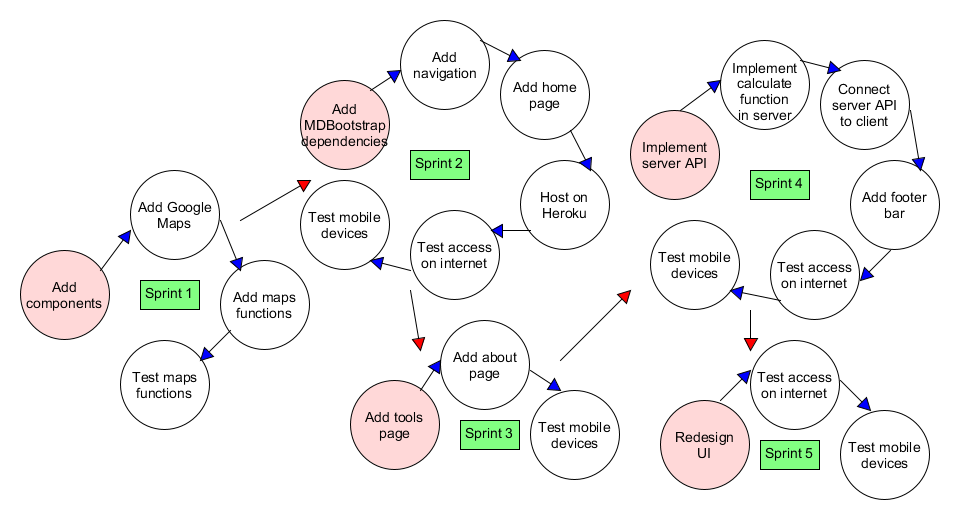
\includegraphics[scale=0.4]{sprints_diagram.png}
		\caption{A simplified diagram of each sprints of the project.}
		\label{sprints:1}
	\end{minipage}
\end{figure}

\hyperref[sprints:1]{Figure (1.1)} shows a simplified version of the development life cycle of the project. In sprint 2 after adding a home page to the application, I host it on Heroku \cite{WEBSITE_HEROKU:1}. I then wanted to test that the new features I've added to the application works by testing it. I test and verify Re10 to see that I can access it on the internet by going into my internet browser (Google Chrome \cite{WEBSITE_GOOGLE_CHROME:1}) and going to the application URL. I then test and verify Re8 to see that the application can be use on mobile devices by going onto my phone's (iPhone 5 \cite{WEBSITE_WIKIPEDIA_APPLE_IPHONE5:1}) internet browser (Google Chrome) and going to the application URL.


%%%%%%%%%%%%%%%%%%%%%%%%%%%%%%%%%%%%%%%%%%%%%%%%%%%%%%%%%%%%%%%%%%%%%%%%

\chapter{Test Report}
% Report the outcomes of the planned tests here, combining a description of the tests with their results, comparing them to their expected performance. Indicate whether your testing criteria were achieved.

\section{Unit Testing}

\addvbuffer[12pt 8pt]{
	\begin{tabular}{ |p{1cm}||p{12.43cm}| }
		\hline
		\multicolumn{2}{|c|}{\textbf{Test Sample Cases List}} \\
		\hline
		\textbf{ID} & \textbf{How the data will be collected} \\
		\hline
		Re0 & By checking that the web application displays a graphical map (Google Maps). \\
		\hline
		Re2 & Check that the app page has input options for longitude and latitude coordinates. \\
		\hline
		Re5 & Check the app page to see that a result is shown there. \\
		\hline
\end{tabular}}
\textbf{Re0 Display graphical map}

To test that a graphical map can be display in the application, I go to the page in which the map (Angular Google Maps \cite{WEBSITE_GOOGLE_MAPS:1} \cite{WEBSITE_AGM:1}) is implemented in and check to see that the map is displayed there.
\\\\
\textbf{Re2 Have coordinates user input}

On the same html page as the graphical map is a form with 2 number input fields, and submit buttons (show the coordinates on the map, and calculate the surface area using the coordinates). I check that I can input latitude and longitude coordinates into the field and submit it using the buttons.

To verified that the input fields takes coordinates I try to enter other characters that are not integers ('1', '2', '3' ..), plus sign ('+'), minus sign ('-'), and decimal point ('.'). Other characters were unable to be inputted into the fields, because the fields are specified as type "number" only. This prevent input coordinates error.

When invalid coordinates are inputted, e.g. latitude = 212313, longitude = 123123, the map does not load any location (grey background) and the surface area result is 0. 

I'm considering that in future iteration of the application I implement an input verifier to check that the input latitude (lat) and longitude (lng) are valid coordinates. This might be able to achieve by restraining the lat between known min and max value of lat, and lng vice versa.
\\\\
\textbf{Re5 Display surface area result}

I go to the html page where the calculation function is located, select/input a coordinates and click on calculate. I then check that the result of the calculation is shown on the page.

To check that the result is actually the total surface area, I logged the result of the calculation in the server, and compare it with the result shown on the web page.

\section{System Testing}

\addvbuffer[12pt 8pt]{
	\begin{tabular}{ |p{1cm}||p{12.43cm}| }
		\hline
		\multicolumn{2}{|c|}{\textbf{Test Sample Cases List}} \\
		\hline
		\textbf{ID} & \textbf{How the data will be collected} \\
		\hline
		Re1 & Interact with the map on the web application page. Interaction includes scrolling to zoom in and out, dragging to move around the map, clicking on the map to add a marker and centre the map on the added marker, change map type and style, dragging a marker, clicking on a marker to show more info. \\
		\hline
		Re3 & Click on the "show on map" button to test the functionality. Check that a new marker is added on the map. Check that the coordinatse of the new marker is the same as the user input coordinates by clicking on the marker to show the marker info which includes its coordinates. \\
		\hline
		Re4 & Check that the map area to calculate is 1 $km^2$. Check that the result is a correct estimate. \\
		\hline
		Re6 & Check that the app doesn't take more than 5 seconds to calculate and return the result, by timing the calculate function. \\
		\hline
		Re7 & Change the size of the web browser on the laptop to see if web app is responsive. Change the size of the mobile device in chrome developer tools\cite{WEBSITE:3} to see if web app is also responsive to different phone screen size. \\
		\hline
		Re8 & Use chrome developer tools and change to mobile view and check that the web app works on the mobile devices. Using a real physical phone, on the phone web browser go to the web app address and check that the app works on the phone. \\
		\hline
		Re9 & Get a user to use the application and ask for inputs, comments, and opinions afterwards. \\
		\hline
		Re10 & On both a computer and mobile phone, use the web browser and go to the address of the web application and test that the application works by checking all functionalities. \\
		\hline
\end{tabular}}
\underline{\textbf{Integration Testing}}
\\\\
\textbf{Re1 Have user-to-map interaction}

Go through the list of required map interactions and check that each one can be done. I check that the interaction works on both computer internet browser and mobile device internet browser.
\\\\
\textbf{Re3 Turn user input coordinates into marker on the map}

Check that there's a button on the page that takes the form inputs of the coordinates and show it on the map. After clicking the button the map changes its centre view to the new user input coordinates.

To check that the coordinates are correct, I use the Google Maps on the web browser \cite{WEBSITE_GOOGLE_MAPS_WEB:1} and I input the user coordinates there. I check that both map shows the same location.
\\\\
\textbf{Re4 Calculate estimated total surface area of roads in user selected $km^2$ on the map}

I first check that the map area to calculate is 1 $km^2$ by logging the calculating how length of each pixel in metres by using a formula provided on the internet \cite{WEBSITE_GOOGLE_GROUPS_MAPS:1}. Then I create a loop where I change the zoom parameter of the map each iteration and see long the sides (the total length of all pixels in one side) of the maps are. I look for the zoom parameter level where the side's length is closes to 1 $km^2$. Once I've found the closest value, I change the size of the Google Static Image \cite{WEBSITE_GOOGLE_MAPS_STATIC:1} (width x height) to match that of 1 $km^2$.

A problem I encounter during this test was that the maximum image size of the static image for the free Google Maps API plan is 640x640 \cite{WEBSITE_GOOGLE_MAPS_STATIC_SIZE:1}. This was a problem because with the zoom level I had my image set at the number of pixels are more 640x640. To solve this problem I run the image length loop test again and find the number of pixels side that are less than or equal to 640.

In creating a road image of the map, I also take into consideration the Google logo and licensing info watermark at the bottom of the image. To an accurate result of the surface area, I need to ignore the watermarks. I solve this problem by calculating the height from the bottom of the image to the top of the watermarks, lets call this $x$. I then add $2x$ pixels to the height of the image so that the watermark is extended out of the 1 $km^2$ view of the image \hyperref[image:2]{Figure (4.2)}. I then would start my calculation on the first pixel after $x$ height pixels on the top and end on the last pixel before $x$ height pixels from the bottom.

After getting a correct size image of 1 $km^2$ area, I go through each pixel of the image and check whether the pixel is visible or not. I make this check because the style I created the map image with make it so that the map only display roads and nothing else. The image result in only roads having visible pixels (255 alpha value). I use get-pixels \cite{WEBSITE_GET-PIXELS:1} to get the RGBA values of each pixel, and the data structure I traverse through each pixel is done using ndarray \cite{WEBSITE_NDARRAY:1}.

For each pixel that is a road pixel I increment a counter I created representing the number of road pixels in the map 1 $km^2$ area. Once all pixels are check I multiply the road pixels count with the $m^2$ area of the pixel using the same formula as before \cite{WEBSITE_GOOGLE_GROUPS_MAPS:1}, divide it by 1000000 to get the $km^2$ surface area of roads.

This whole calculation process is tested correctly by logging the pixels data structure and its index. I then check the index against my own calculations to make sure that I'm calculating the correct pixels, and not the extending $x$ areas.

My whole work process for setting the image size and calculating the surface area of roads can be found in the \hyperref[chapter:appendix]{Appendix}.
\\\\
\underline{\textbf{System Testing}}
\\\\
\textbf{Re8 Can be use on mobile device}

I test that the application can be use on mobile devices by both using the mobile view in the Google Chrome DevTools \cite{WEBSITE_GOOGLE_CHROME_DEVTOOLS:1}, and by opening the application through the web browser on my mobile phone.
\\\\
\textbf{Re10 Can access the application on the internet}

I test this requirement by going to the application URL address on both my computer and mobile device.
\\\\
\underline{\textbf{Performance Testing}}
\\\\
\textbf{Re6 Doesn't take "long" to do the surface area calculation}

To test the elapsed time the application takes to calculate the surface area, I used the Date object in JavaScript to get the current time before the calculation and then get the current time again after the calculate, and I subtract the after time by the before time to get the calculation elapsed time. The average elapsed time of the calculation is 0.3 seconds.

My calculation of the elapsed time doesn't take into consideration the network speed because it is dynamic and changes with each user, but the calculation speed on the server is less likely to change.

I also display the calculation elapsed time to the user so that they can see how long it takes.
\\\\
\underline{\textbf{Usability Testing}}
\\\\
\textbf{Re7 Web design is responsive}

To test if the the application is responsive I resize the web browser to various sizes to see where the elements end up. I also tested the application on a mobile device view to see if the application is still usable.

I had my friends and family tested the application on their mobile devices to make sure that they are able to use it too, because they have different mobile devices and I wanted to test more devices of different screen sizes.
\\\\
\textbf{Re9 Provide a easy to understand tutorial}

I created a page in the application dedicated as a tutorial page with images of the application and descriptions of its usages.

I had my friends and family test the application by having them go through the tutorial and to tell me if it was easy to understand or not.

The comments that came back was that they like the images that accompanies the descriptive texts. The images next to the text makes it easier to understands and follow.


%%%%%%%%%%%%%%%%%%%%%%%%%%%%%%%%%%%%%%%%%%%%%%%%%%%%%%%%%%%%%%%%%%%%%%%%

\chapter{Conclusion}

All testing that was done in this project was done manually. For future iterations of the projects (and for my own future projects) I will implement a better development operation, where I use automatic testing technologies. Using automatic testing technologies would also encourage me to use Test Driven Development (TDD) more with the project, which leads to me writing better test cases.

%%%%%%%%%%%%%%%%%%%%%%%%%%%%%%%%%%%%%%%%%%%%%%%%%%%%%%%%%%%%%%%%%%%%%%%%

\chapter{Appendix}
\label{chapter:appendix}

\begin{figure}[H]
	\centering
	\begin{minipage}[b]{0.4\textwidth}
		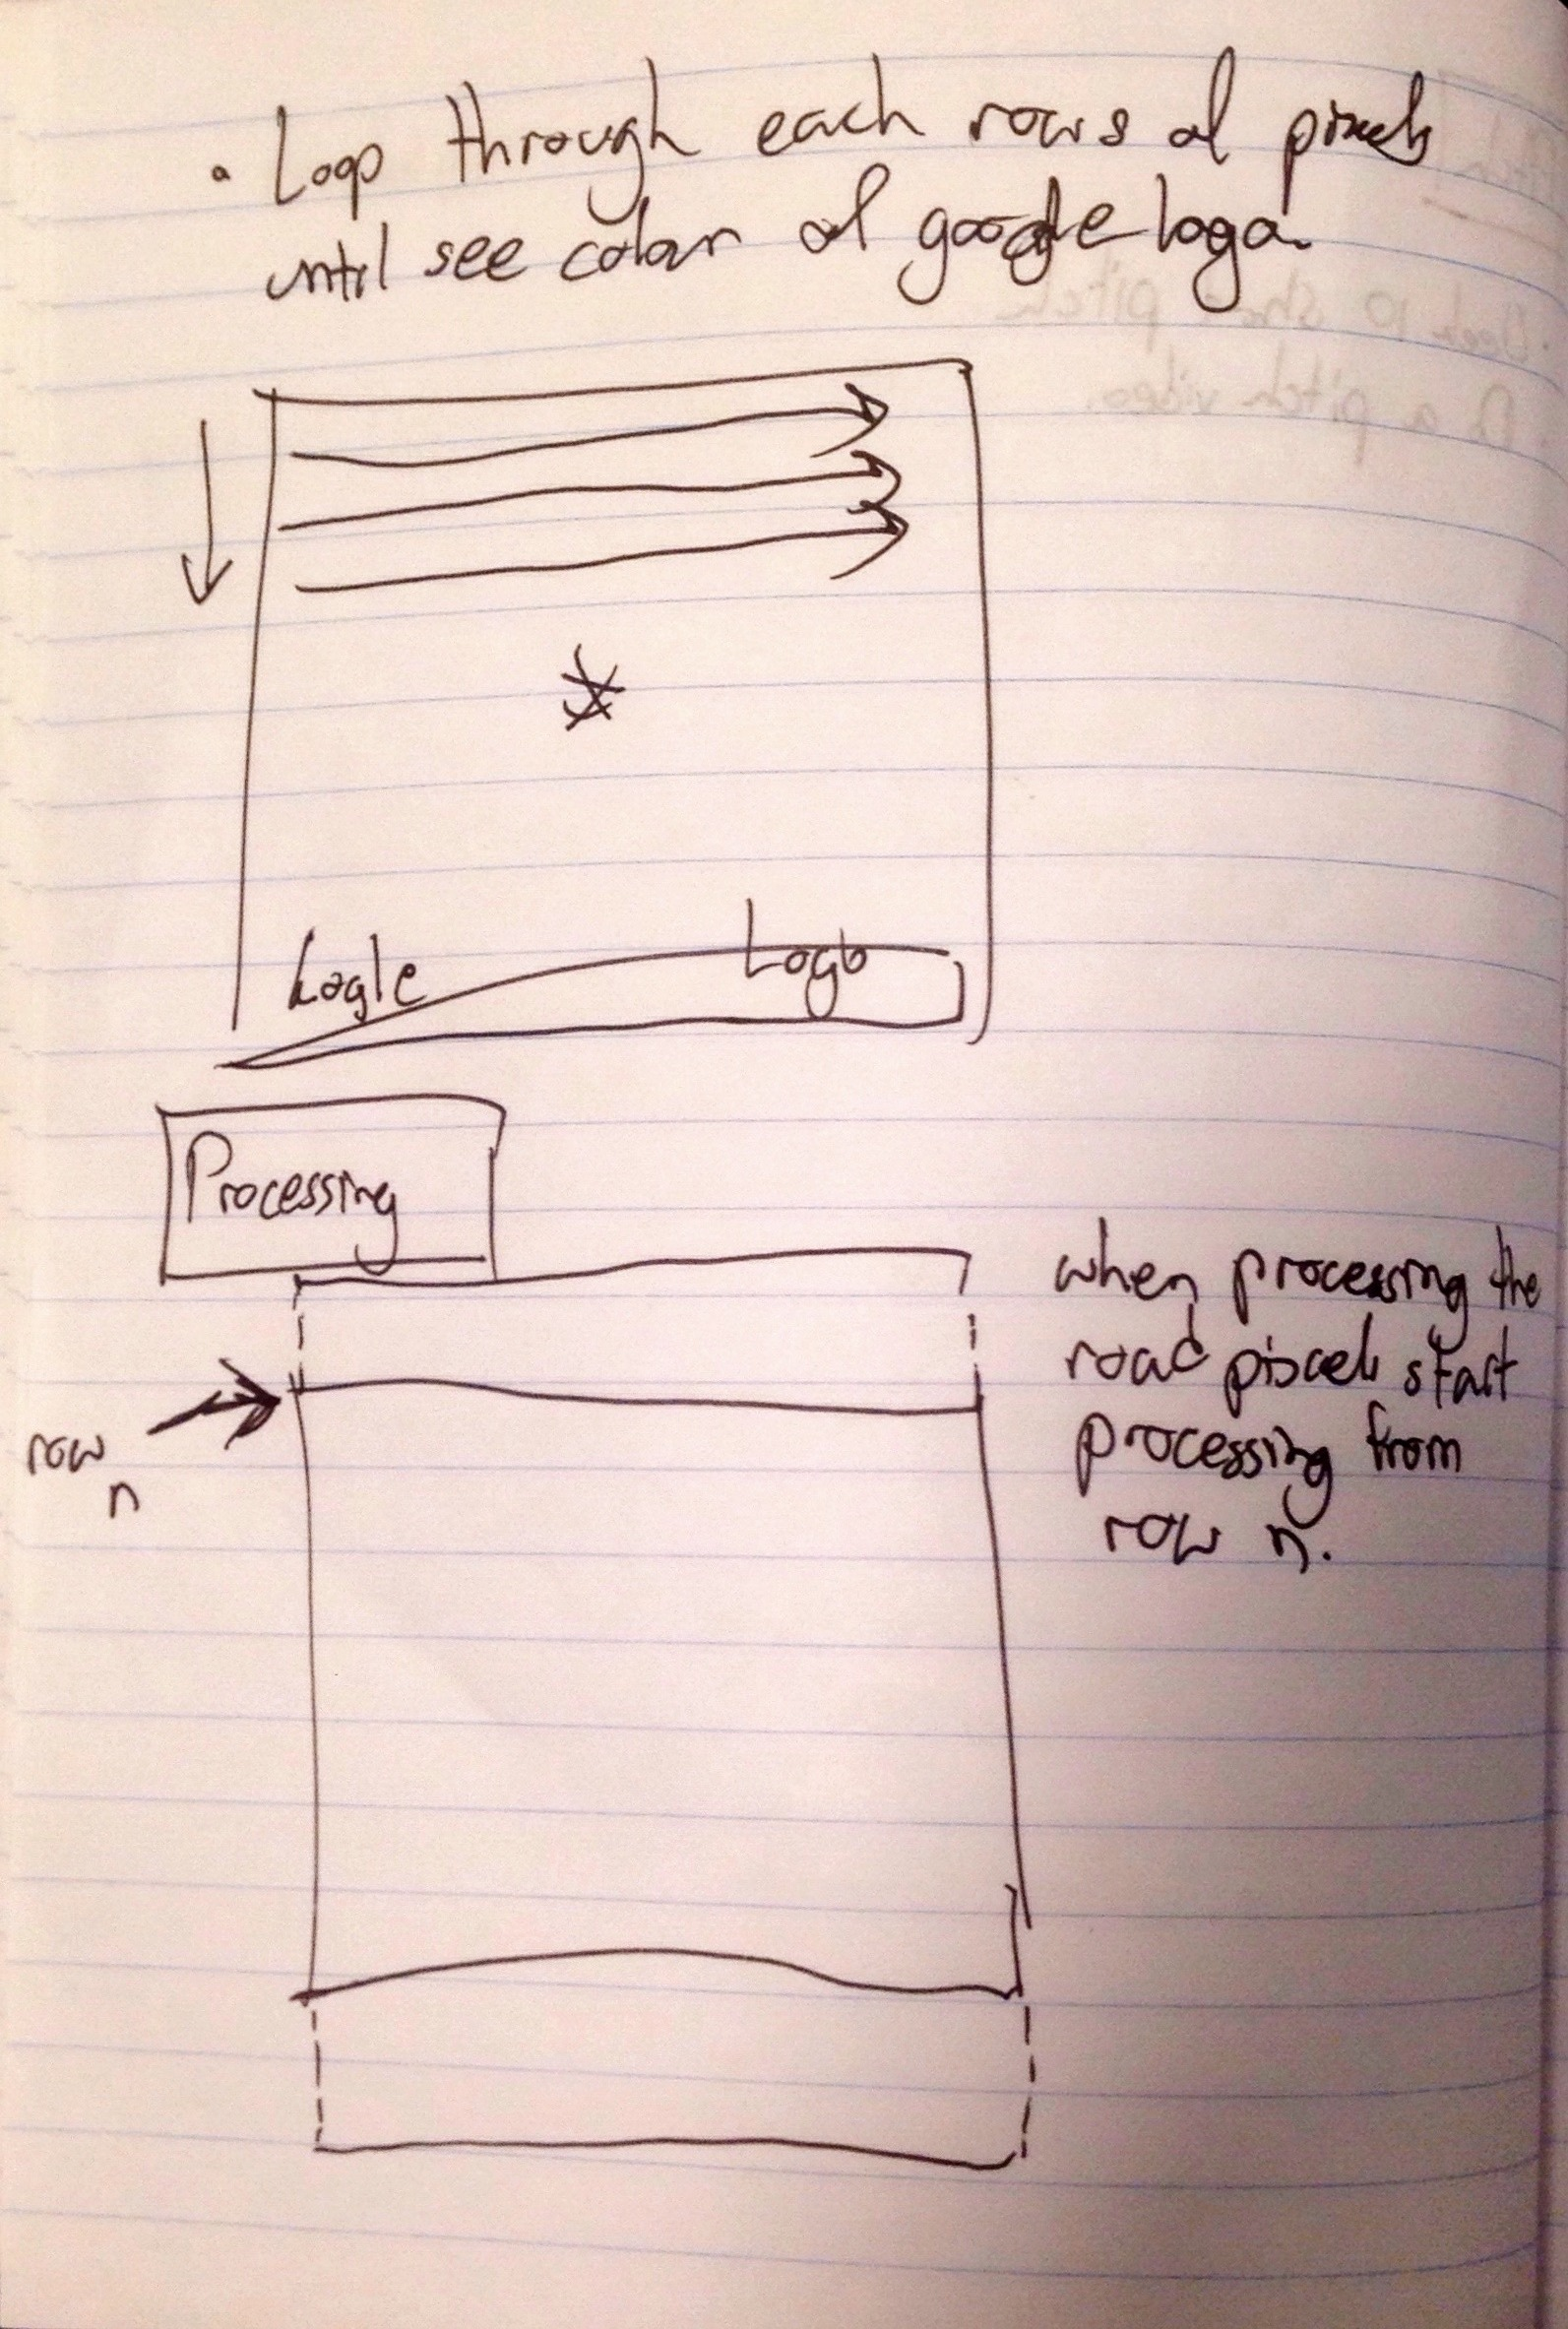
\includegraphics[width=\textwidth]{1.jpg}
		\caption{Image size work process 1.}
	\end{minipage}
	\hfill
	\begin{minipage}[b]{0.4\textwidth}
		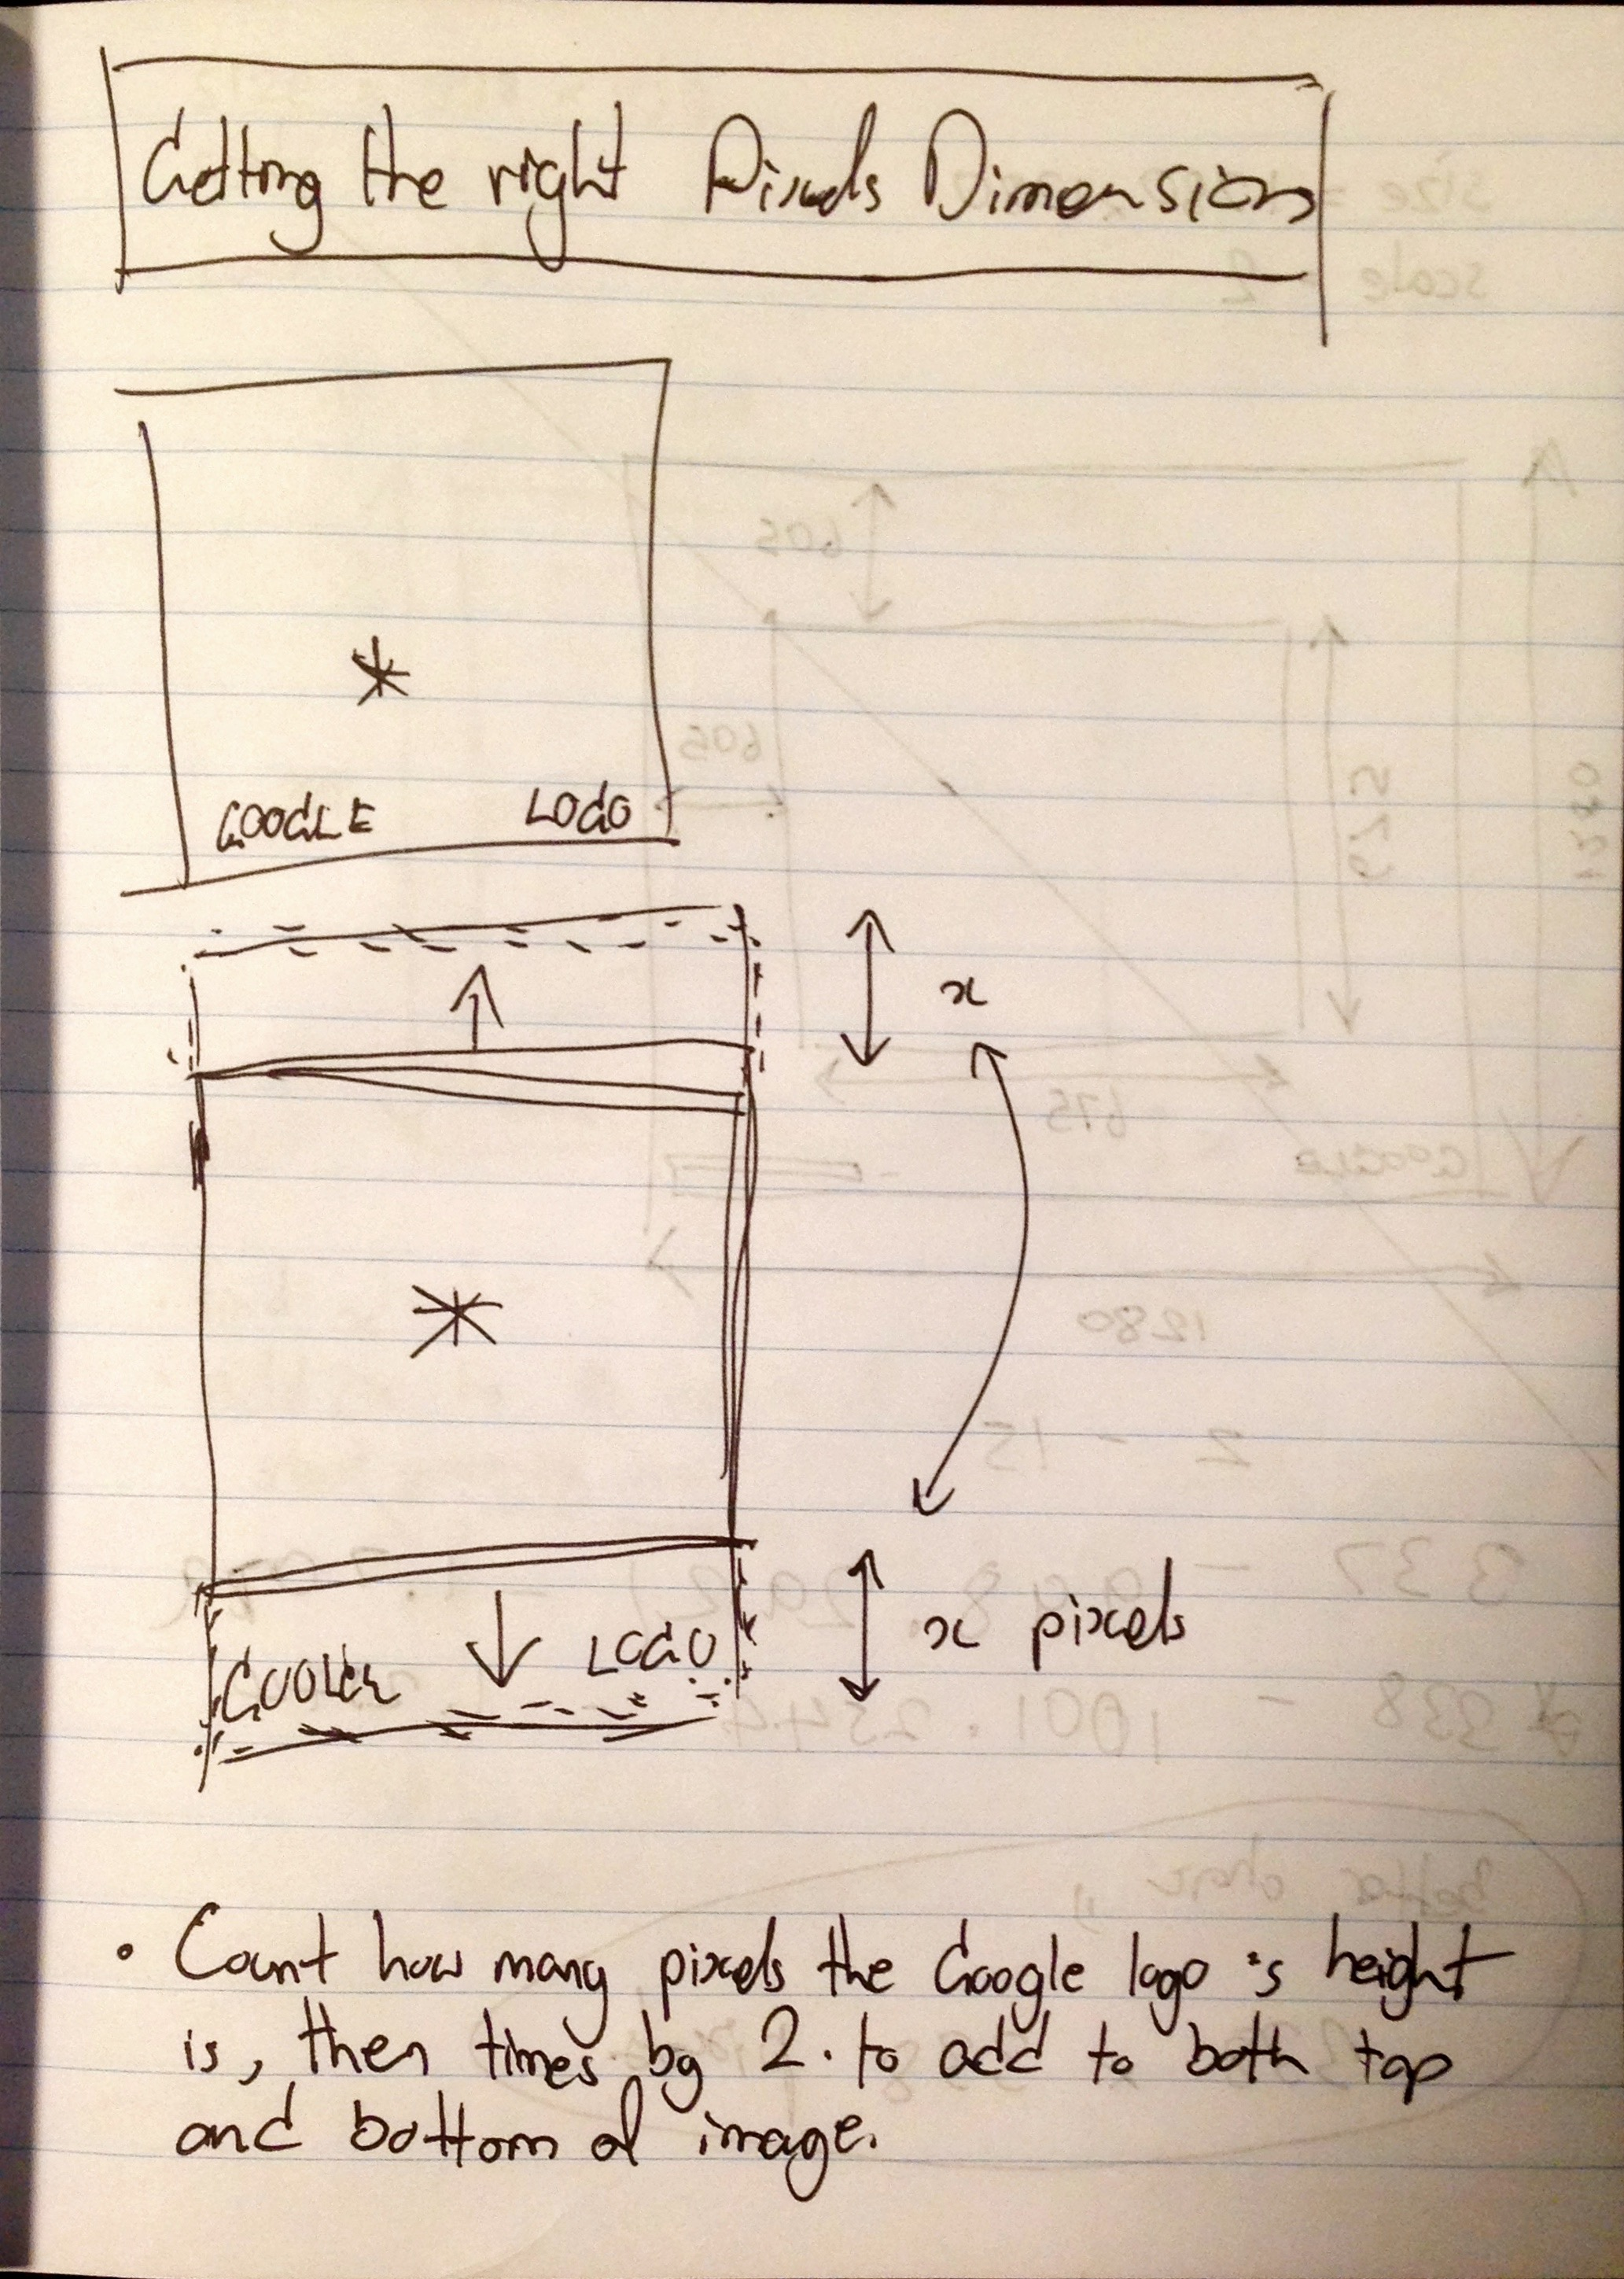
\includegraphics[width=\textwidth]{2.JPG}
		\caption{Image size work process 2.}
		\label{image:2}
	\end{minipage}
\end{figure}

\begin{figure}[H]
	\centering
	\begin{minipage}[b]{0.4\textwidth}
		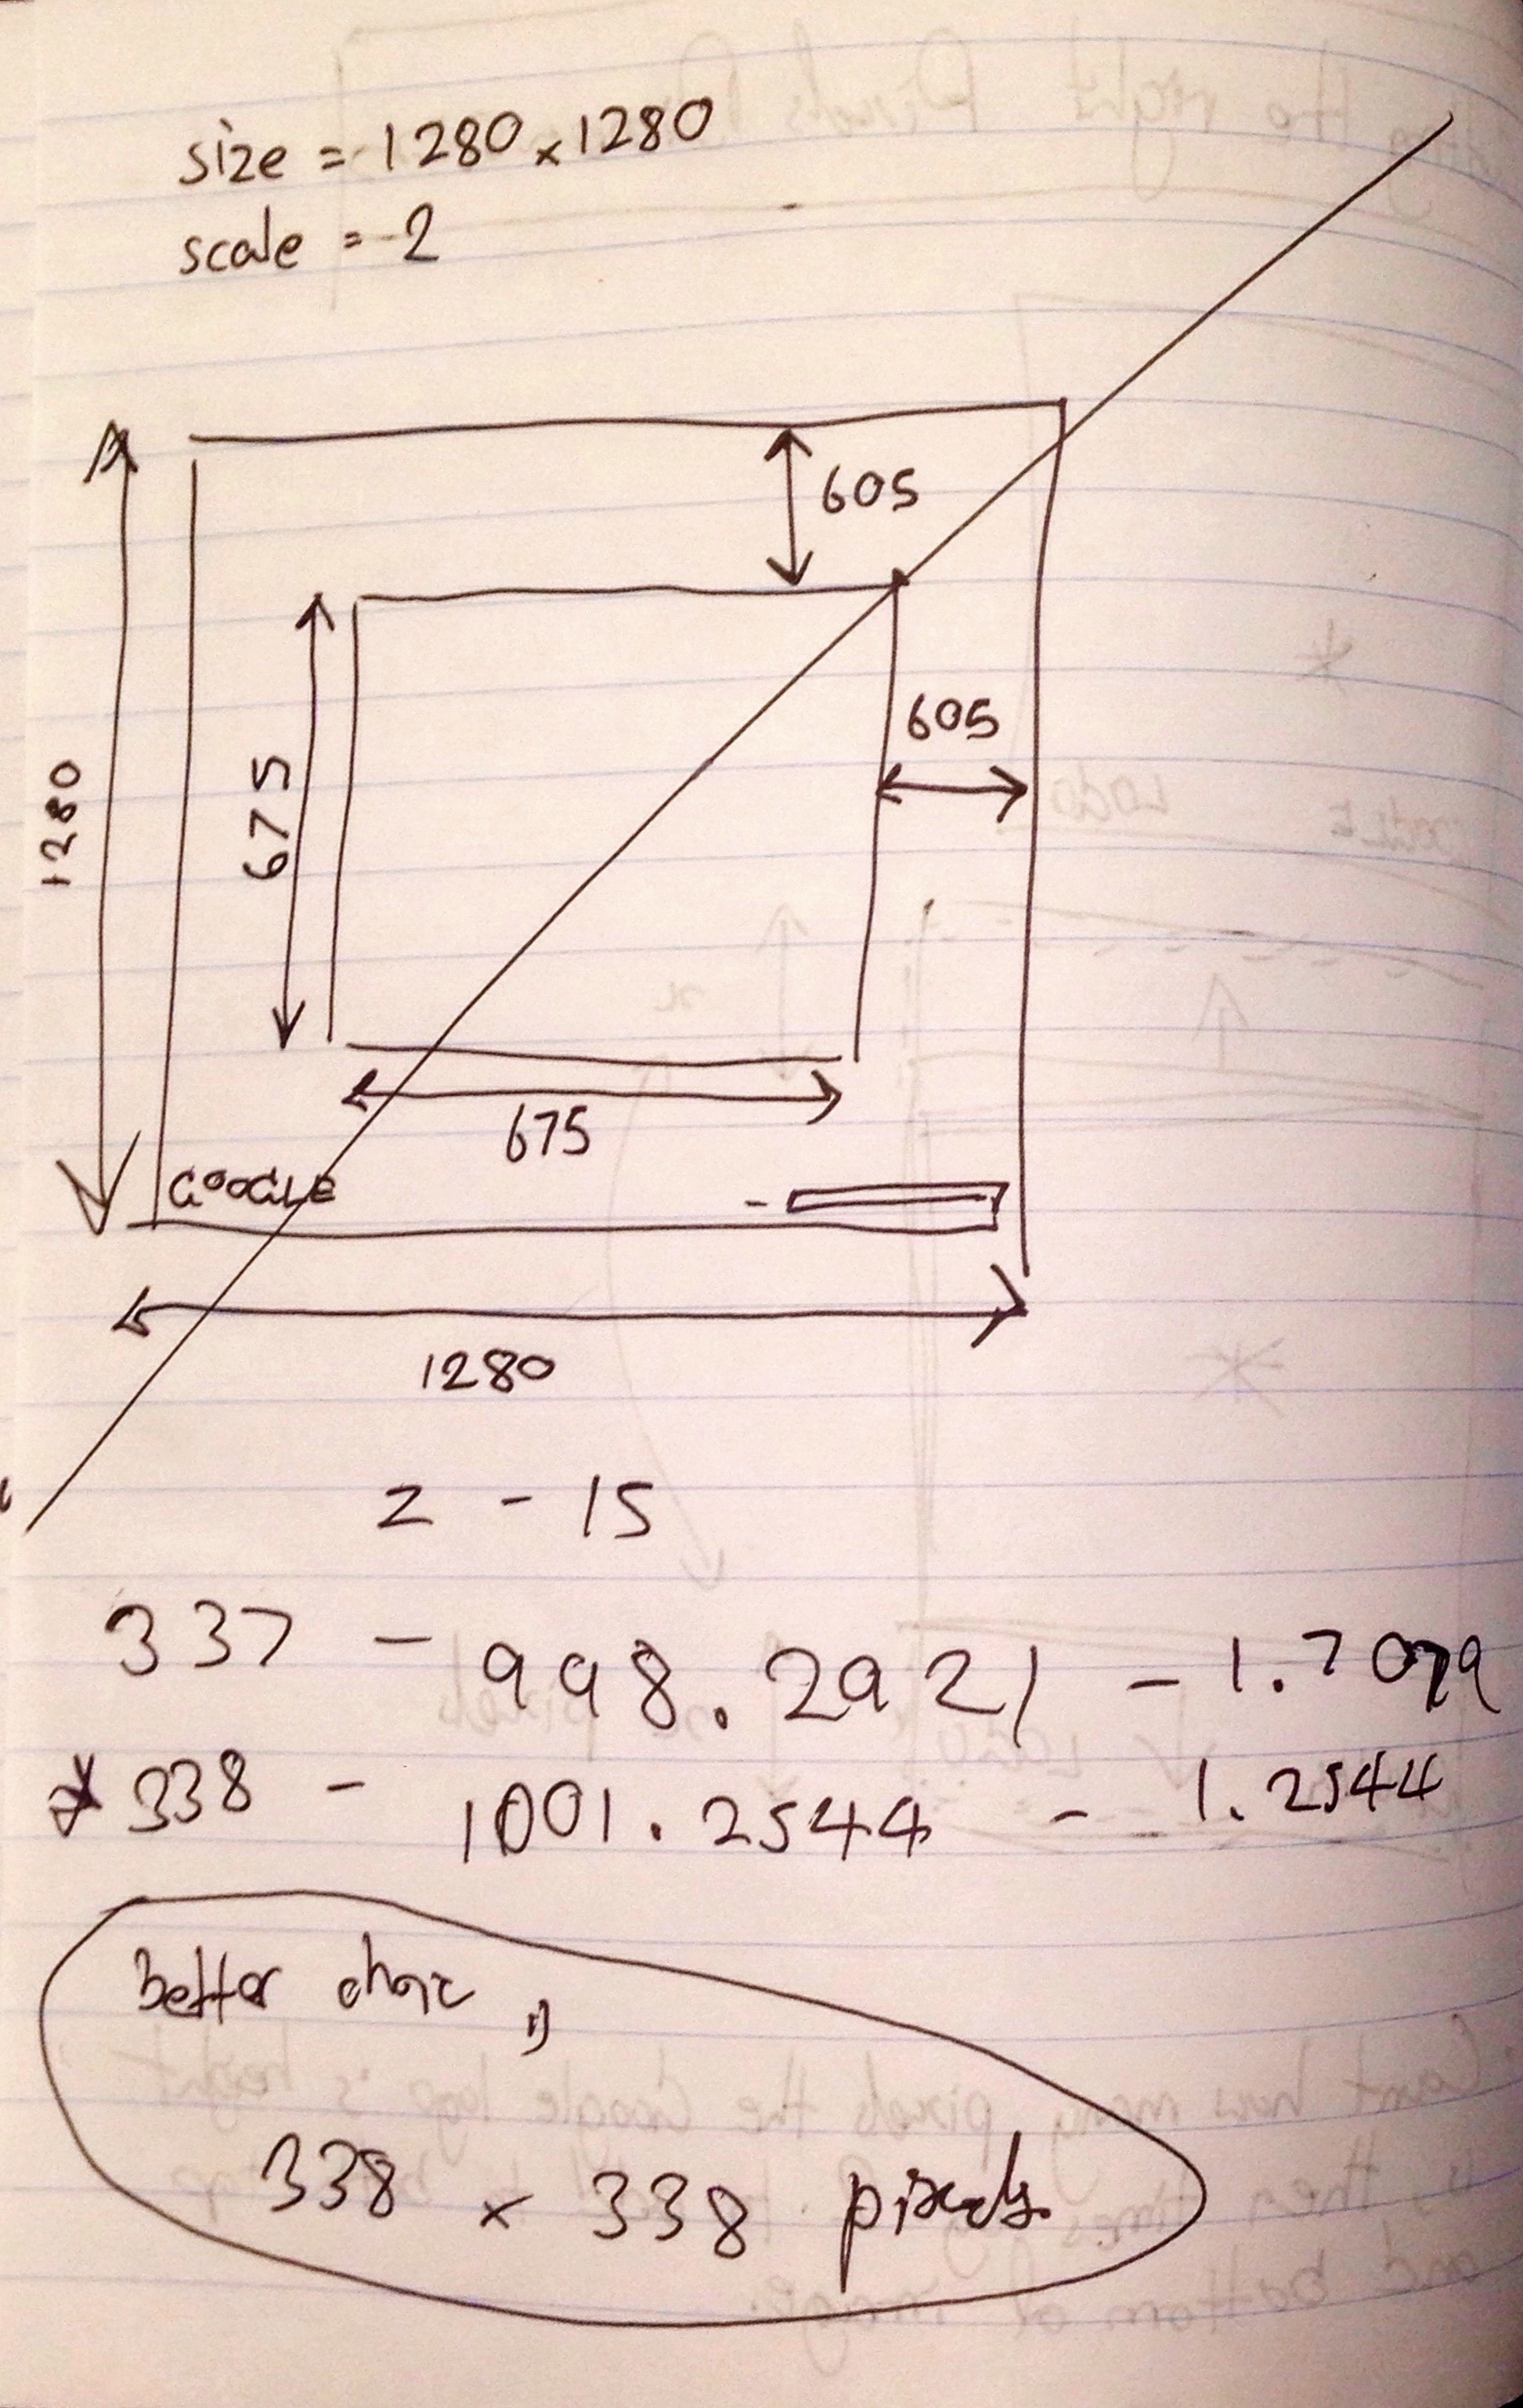
\includegraphics[width=\textwidth]{3.JPG}
		\caption{Image size work process 3.}
	\end{minipage}
	\hfill
	\begin{minipage}[b]{0.4\textwidth}
		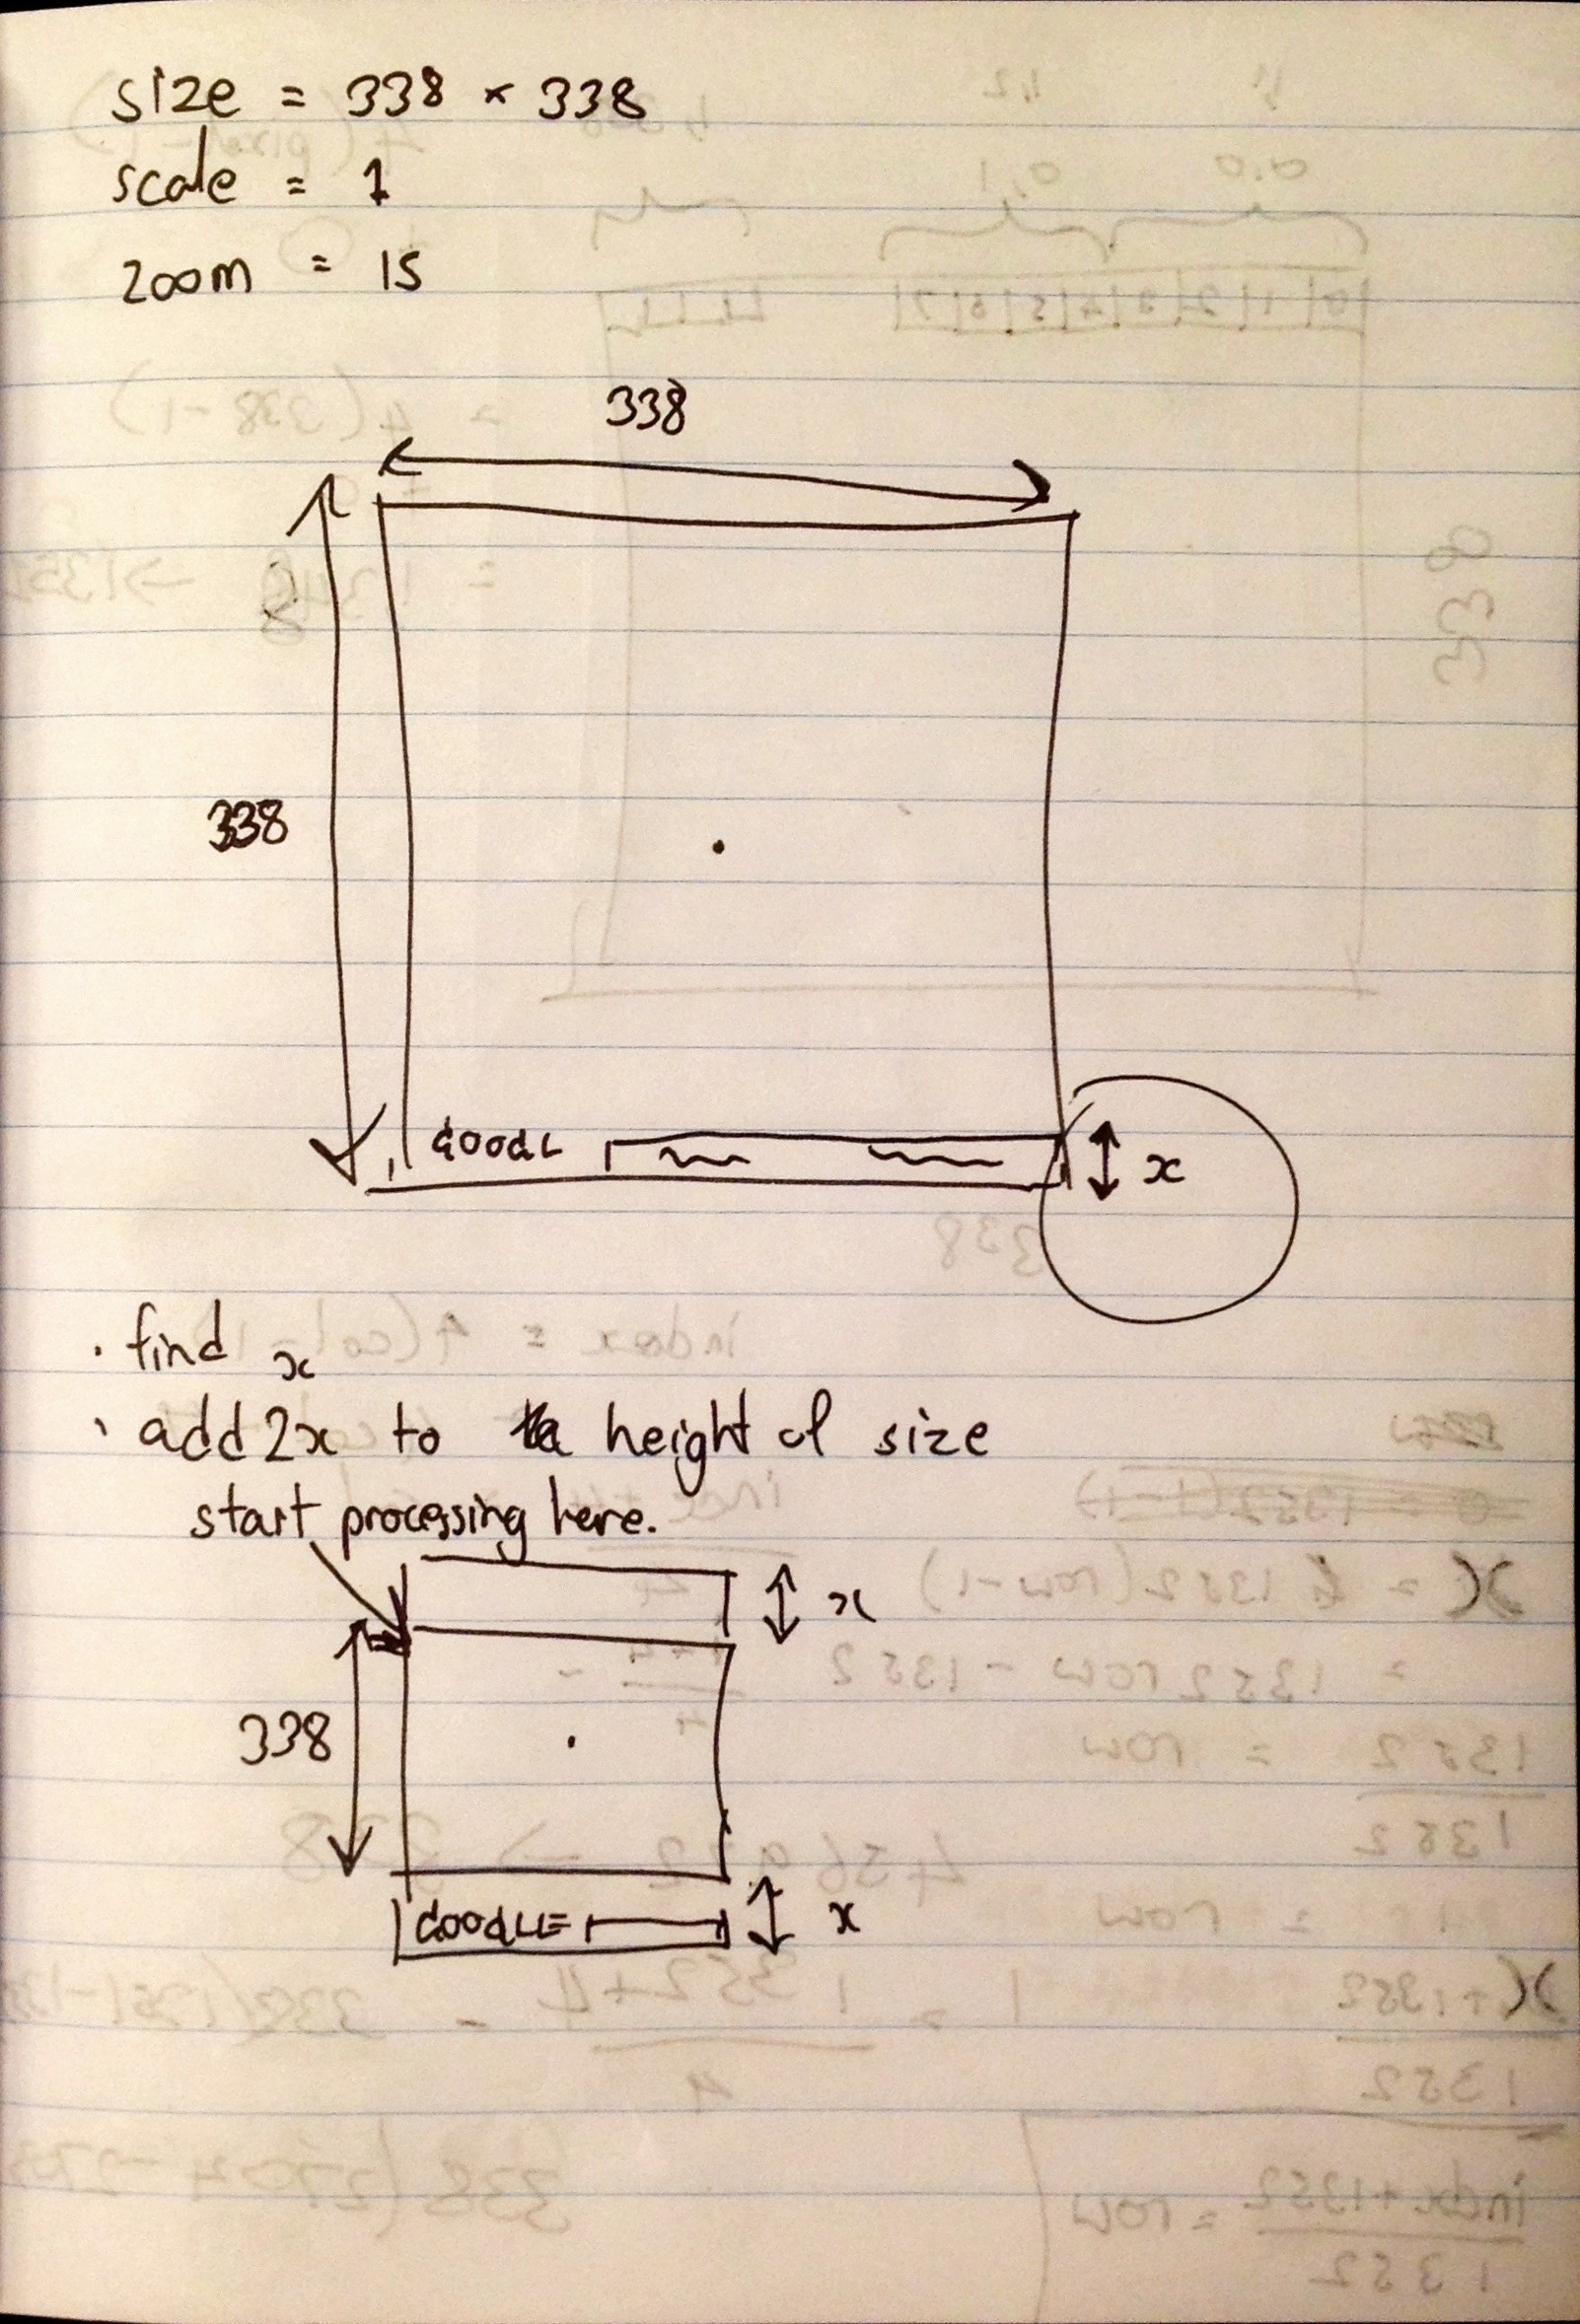
\includegraphics[width=\textwidth]{4.jpg}
		\caption{Image size work process 4.}
	\end{minipage}
\end{figure}

\begin{figure}[H]
	\centering
	\begin{minipage}[b]{0.4\textwidth}
		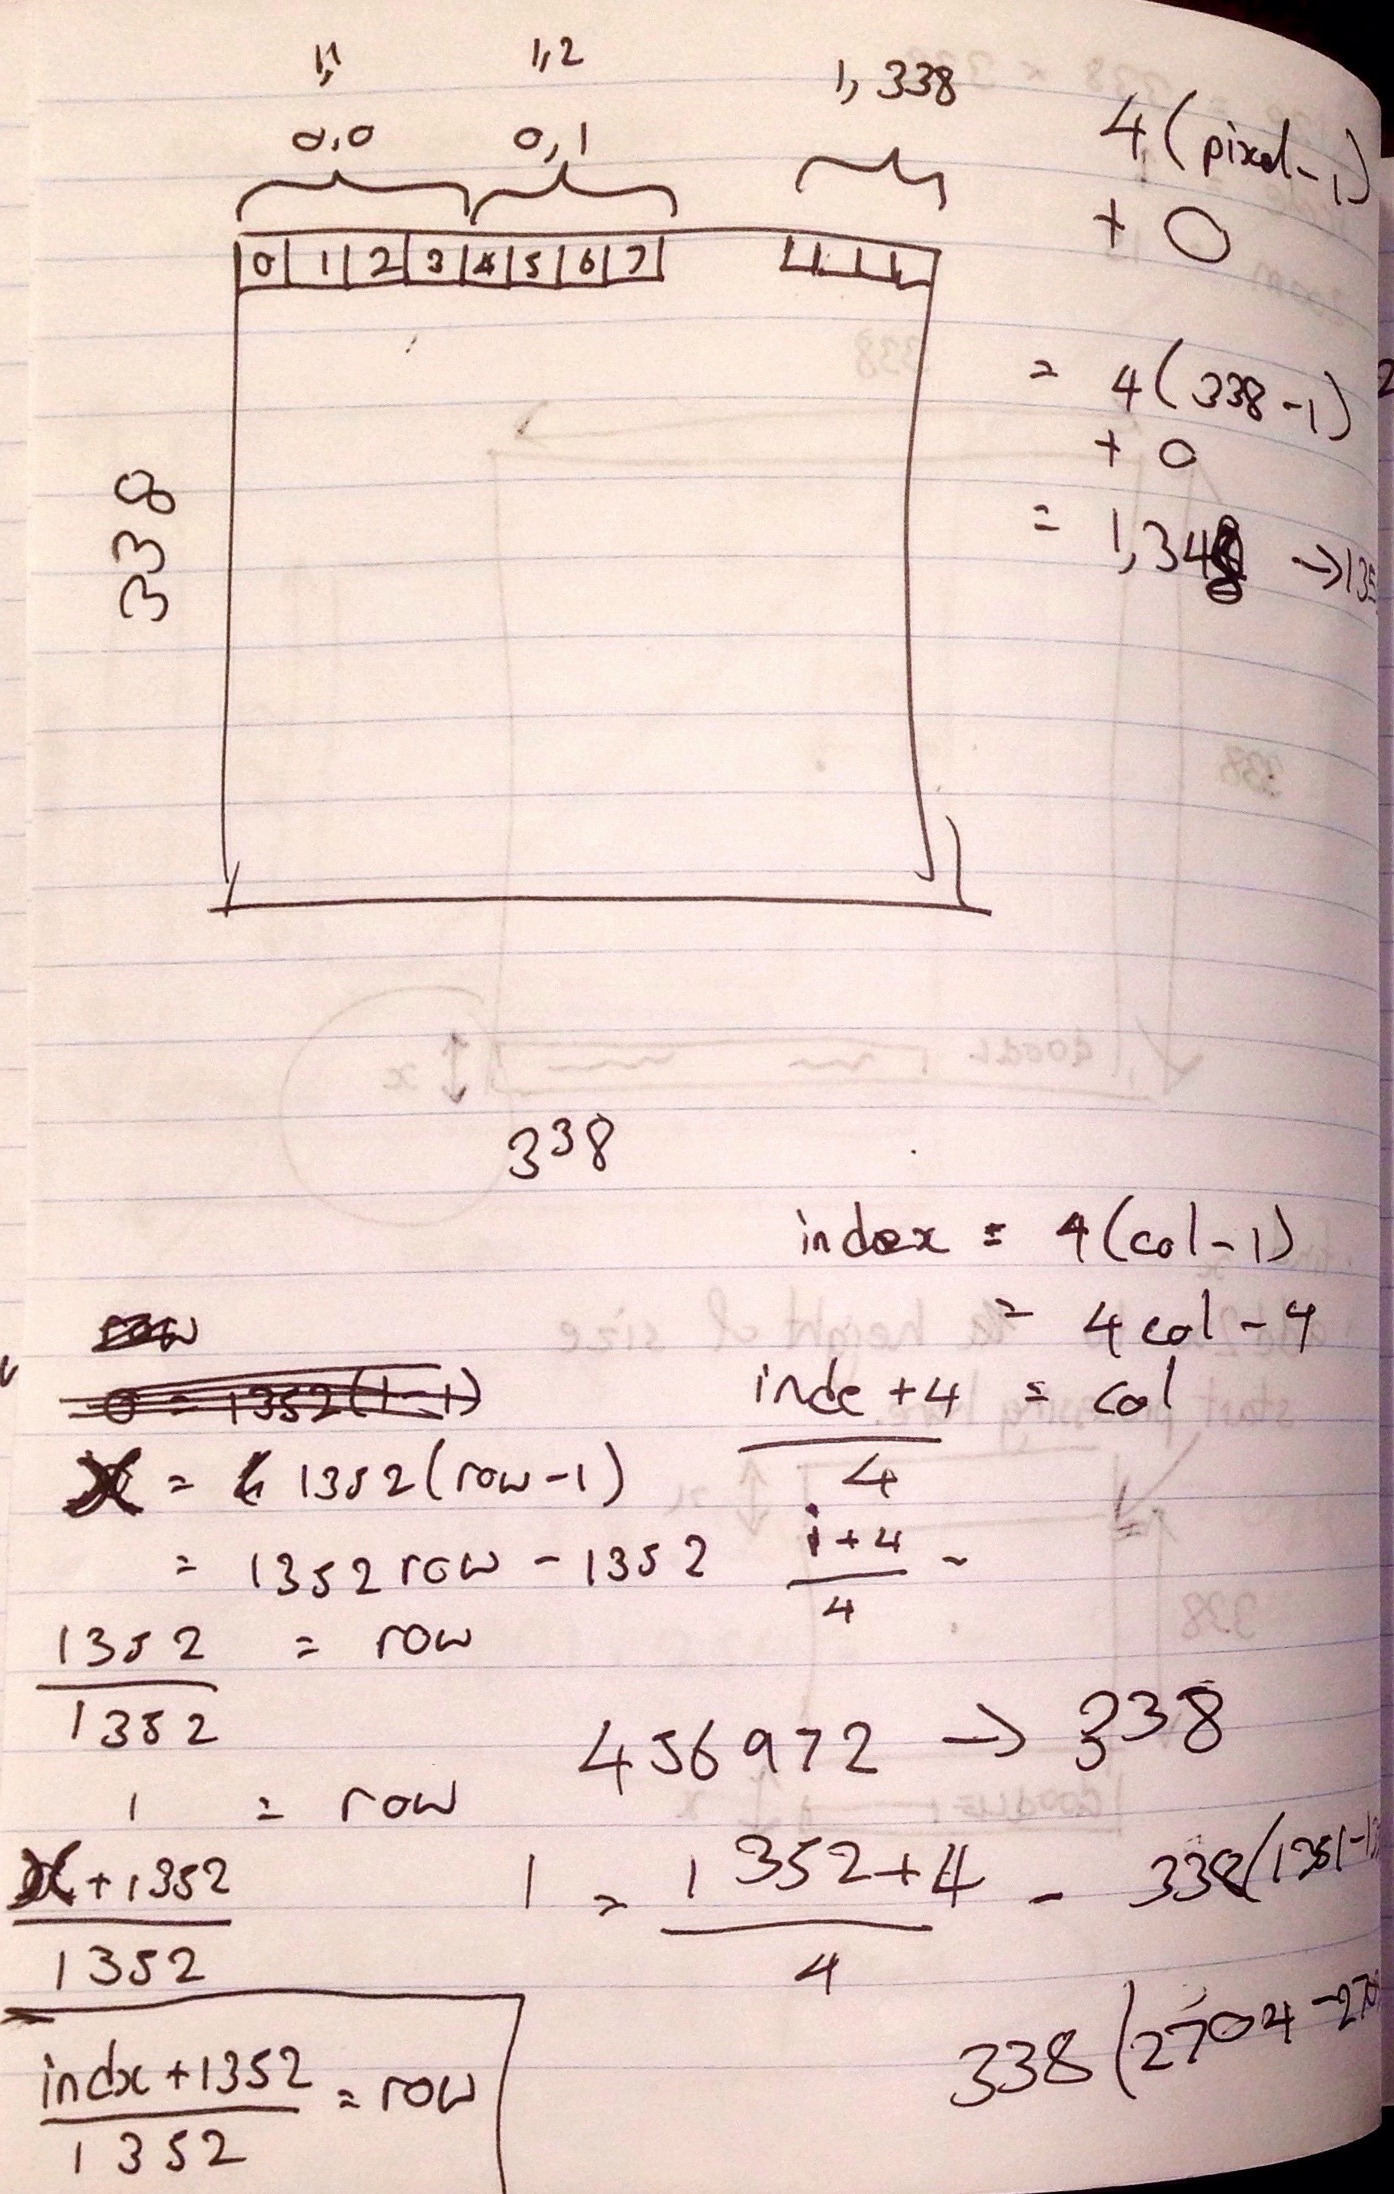
\includegraphics[width=\textwidth]{5.jpg}
		\caption{Image size work process 5.}
	\end{minipage}
	\hfill
	\begin{minipage}[b]{0.4\textwidth}
		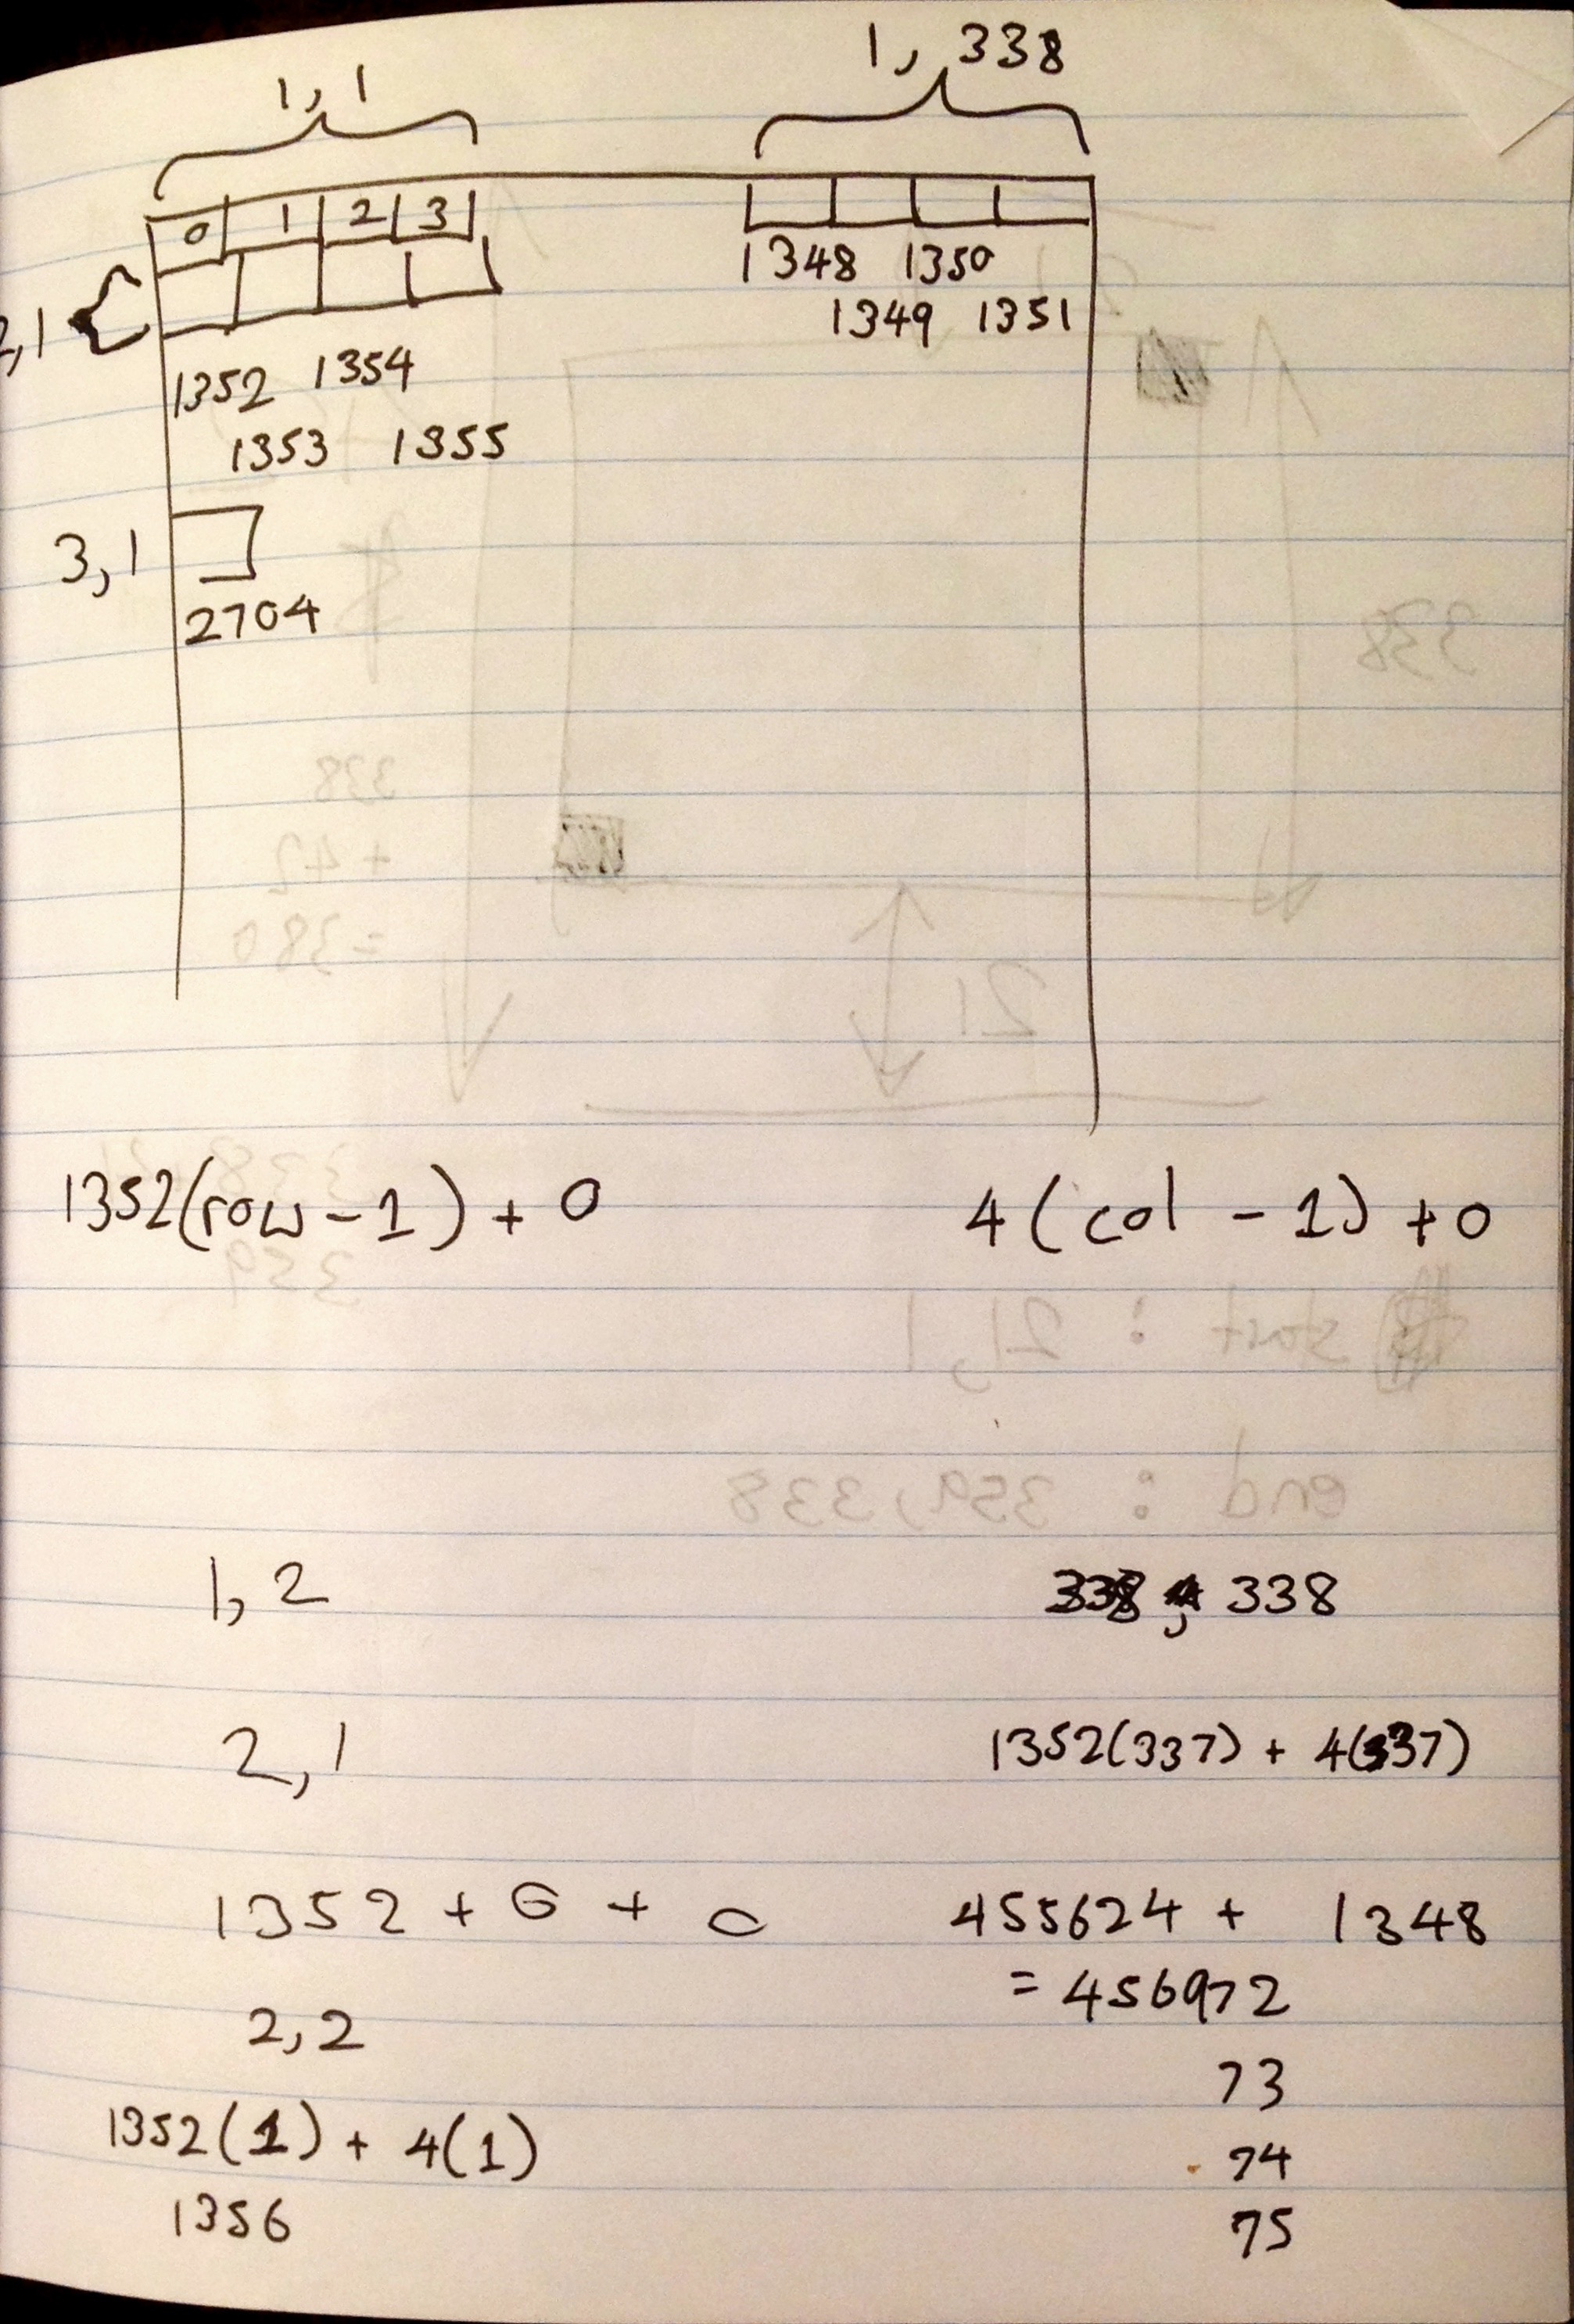
\includegraphics[width=\textwidth]{6.JPG}
		\caption{Image size work process 6.}
	\end{minipage}
\end{figure}

\begin{figure}[H]
	\centering
	\begin{minipage}[b]{0.4\textwidth}
		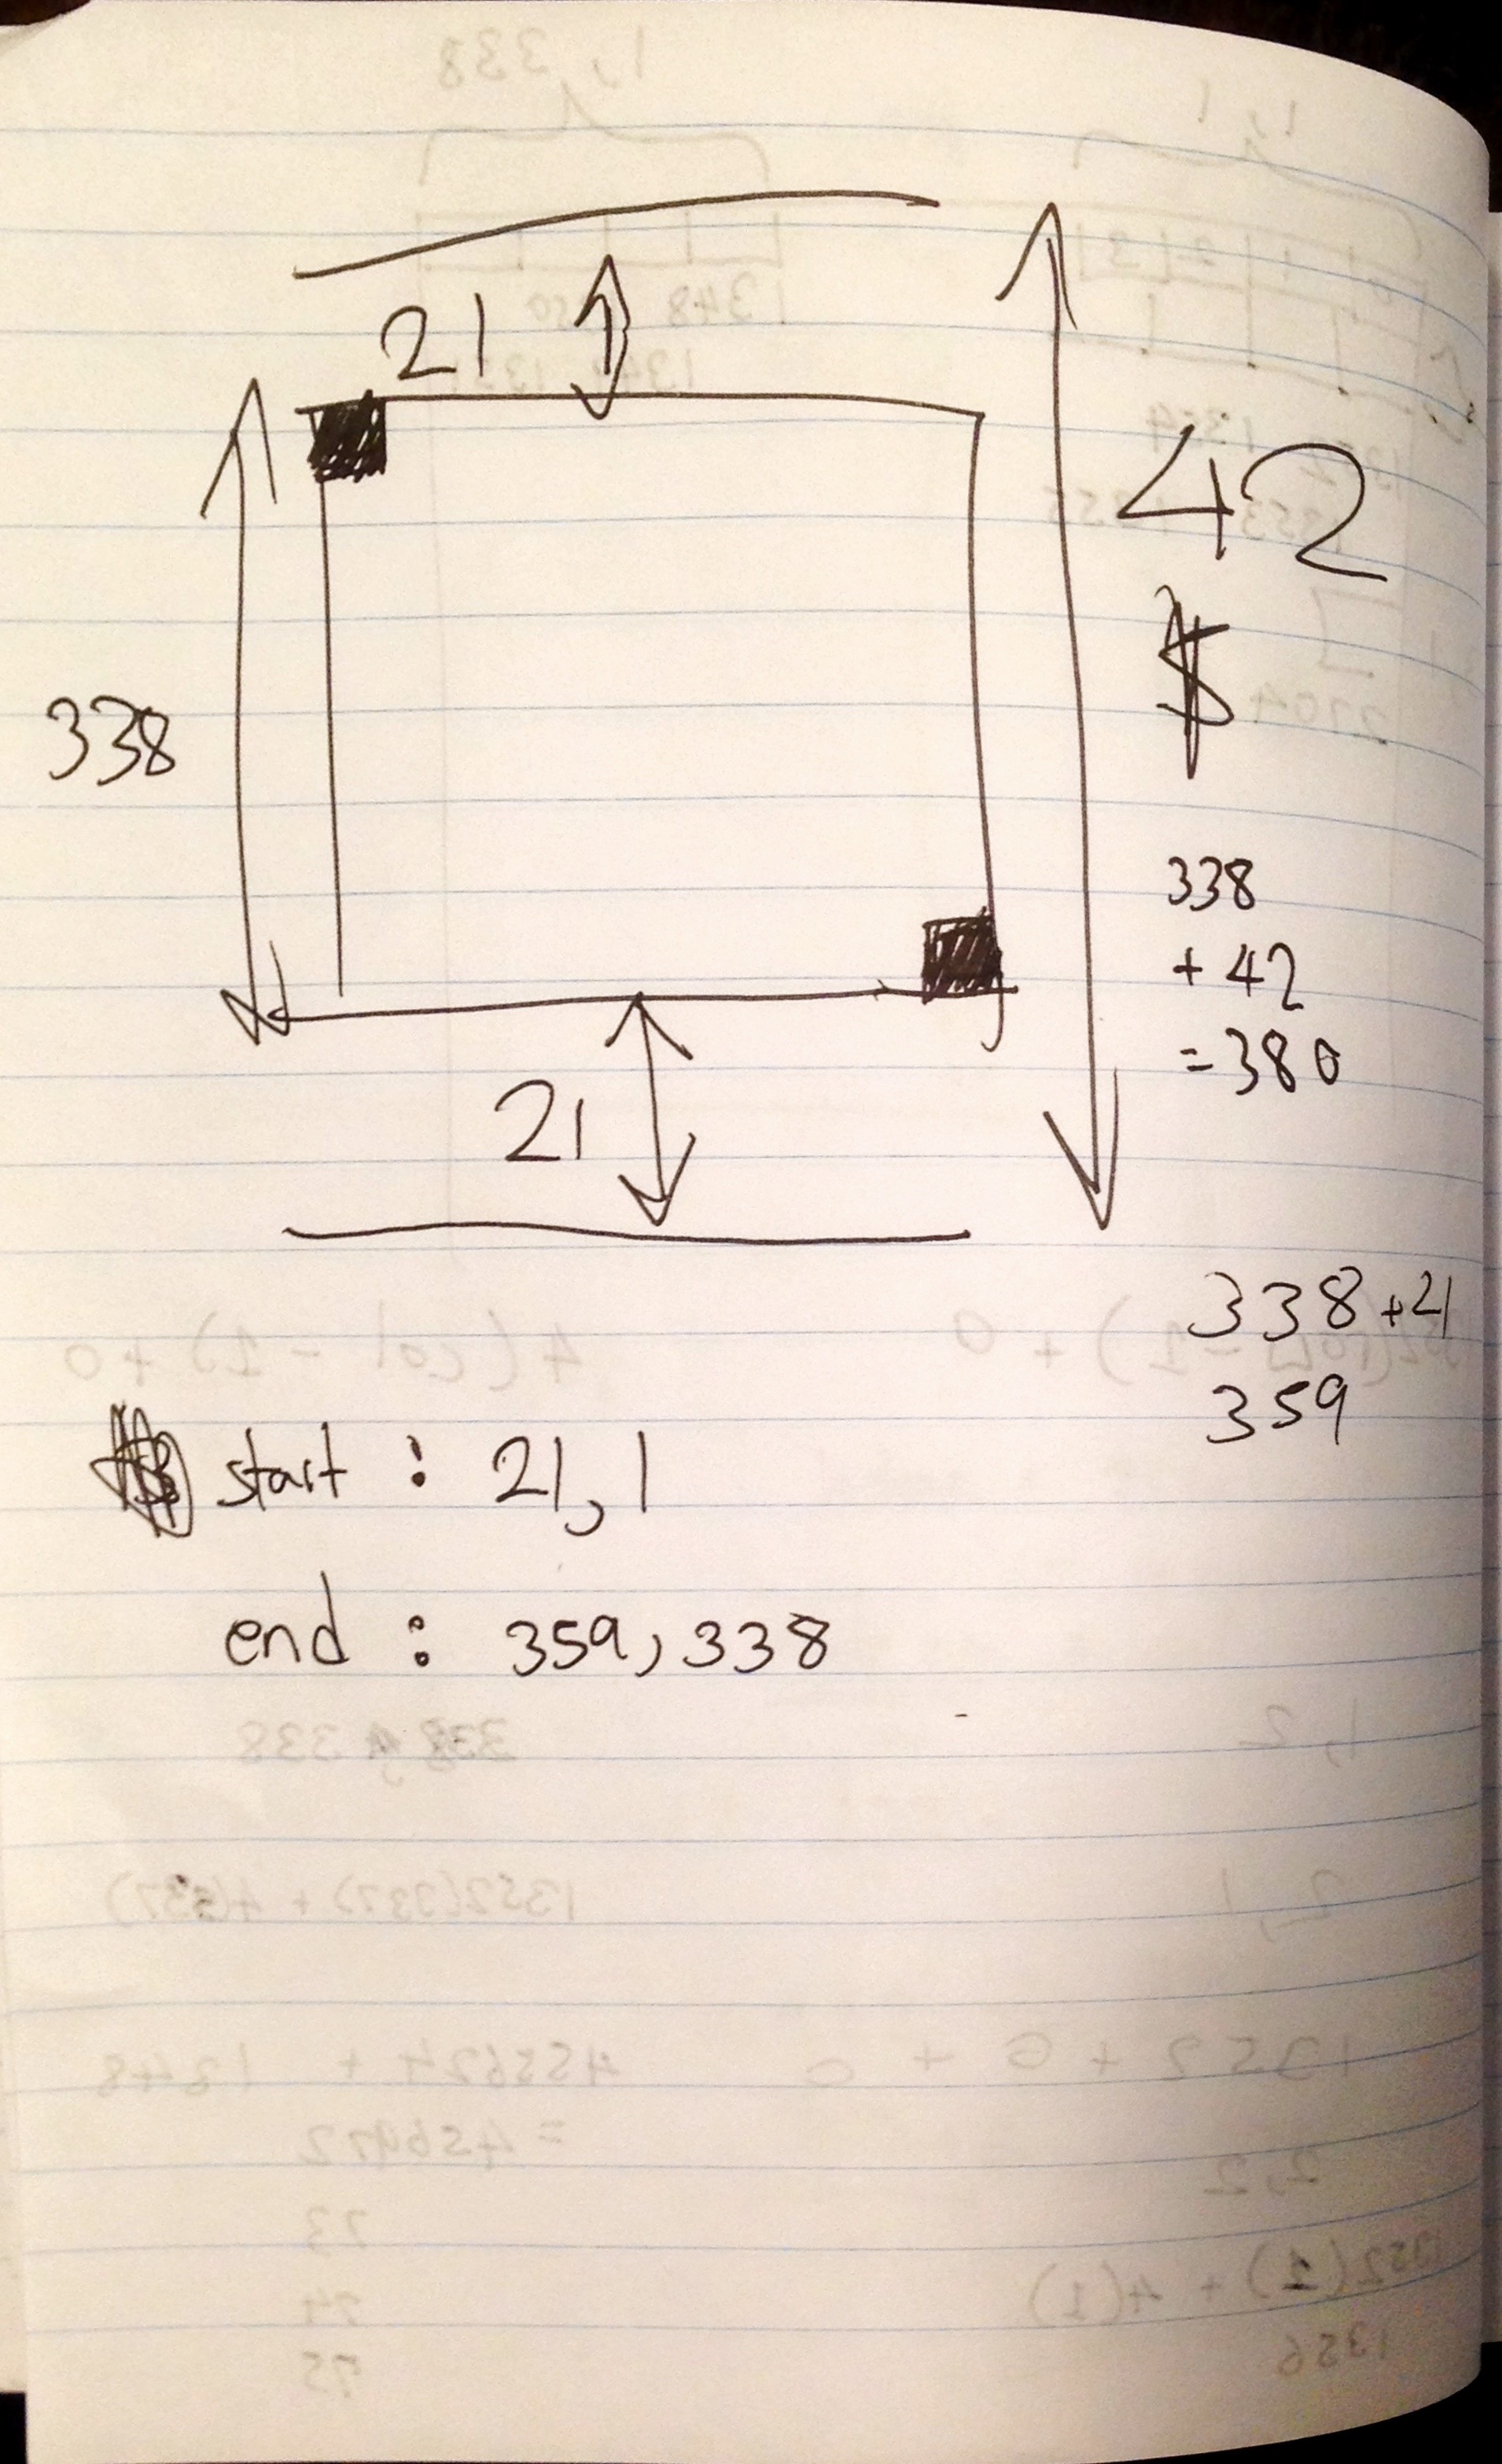
\includegraphics[width=\textwidth]{7.JPG}
		\caption{Image size work process 7.}
	\end{minipage}
	\hfill
	\begin{minipage}[b]{0.4\textwidth}
		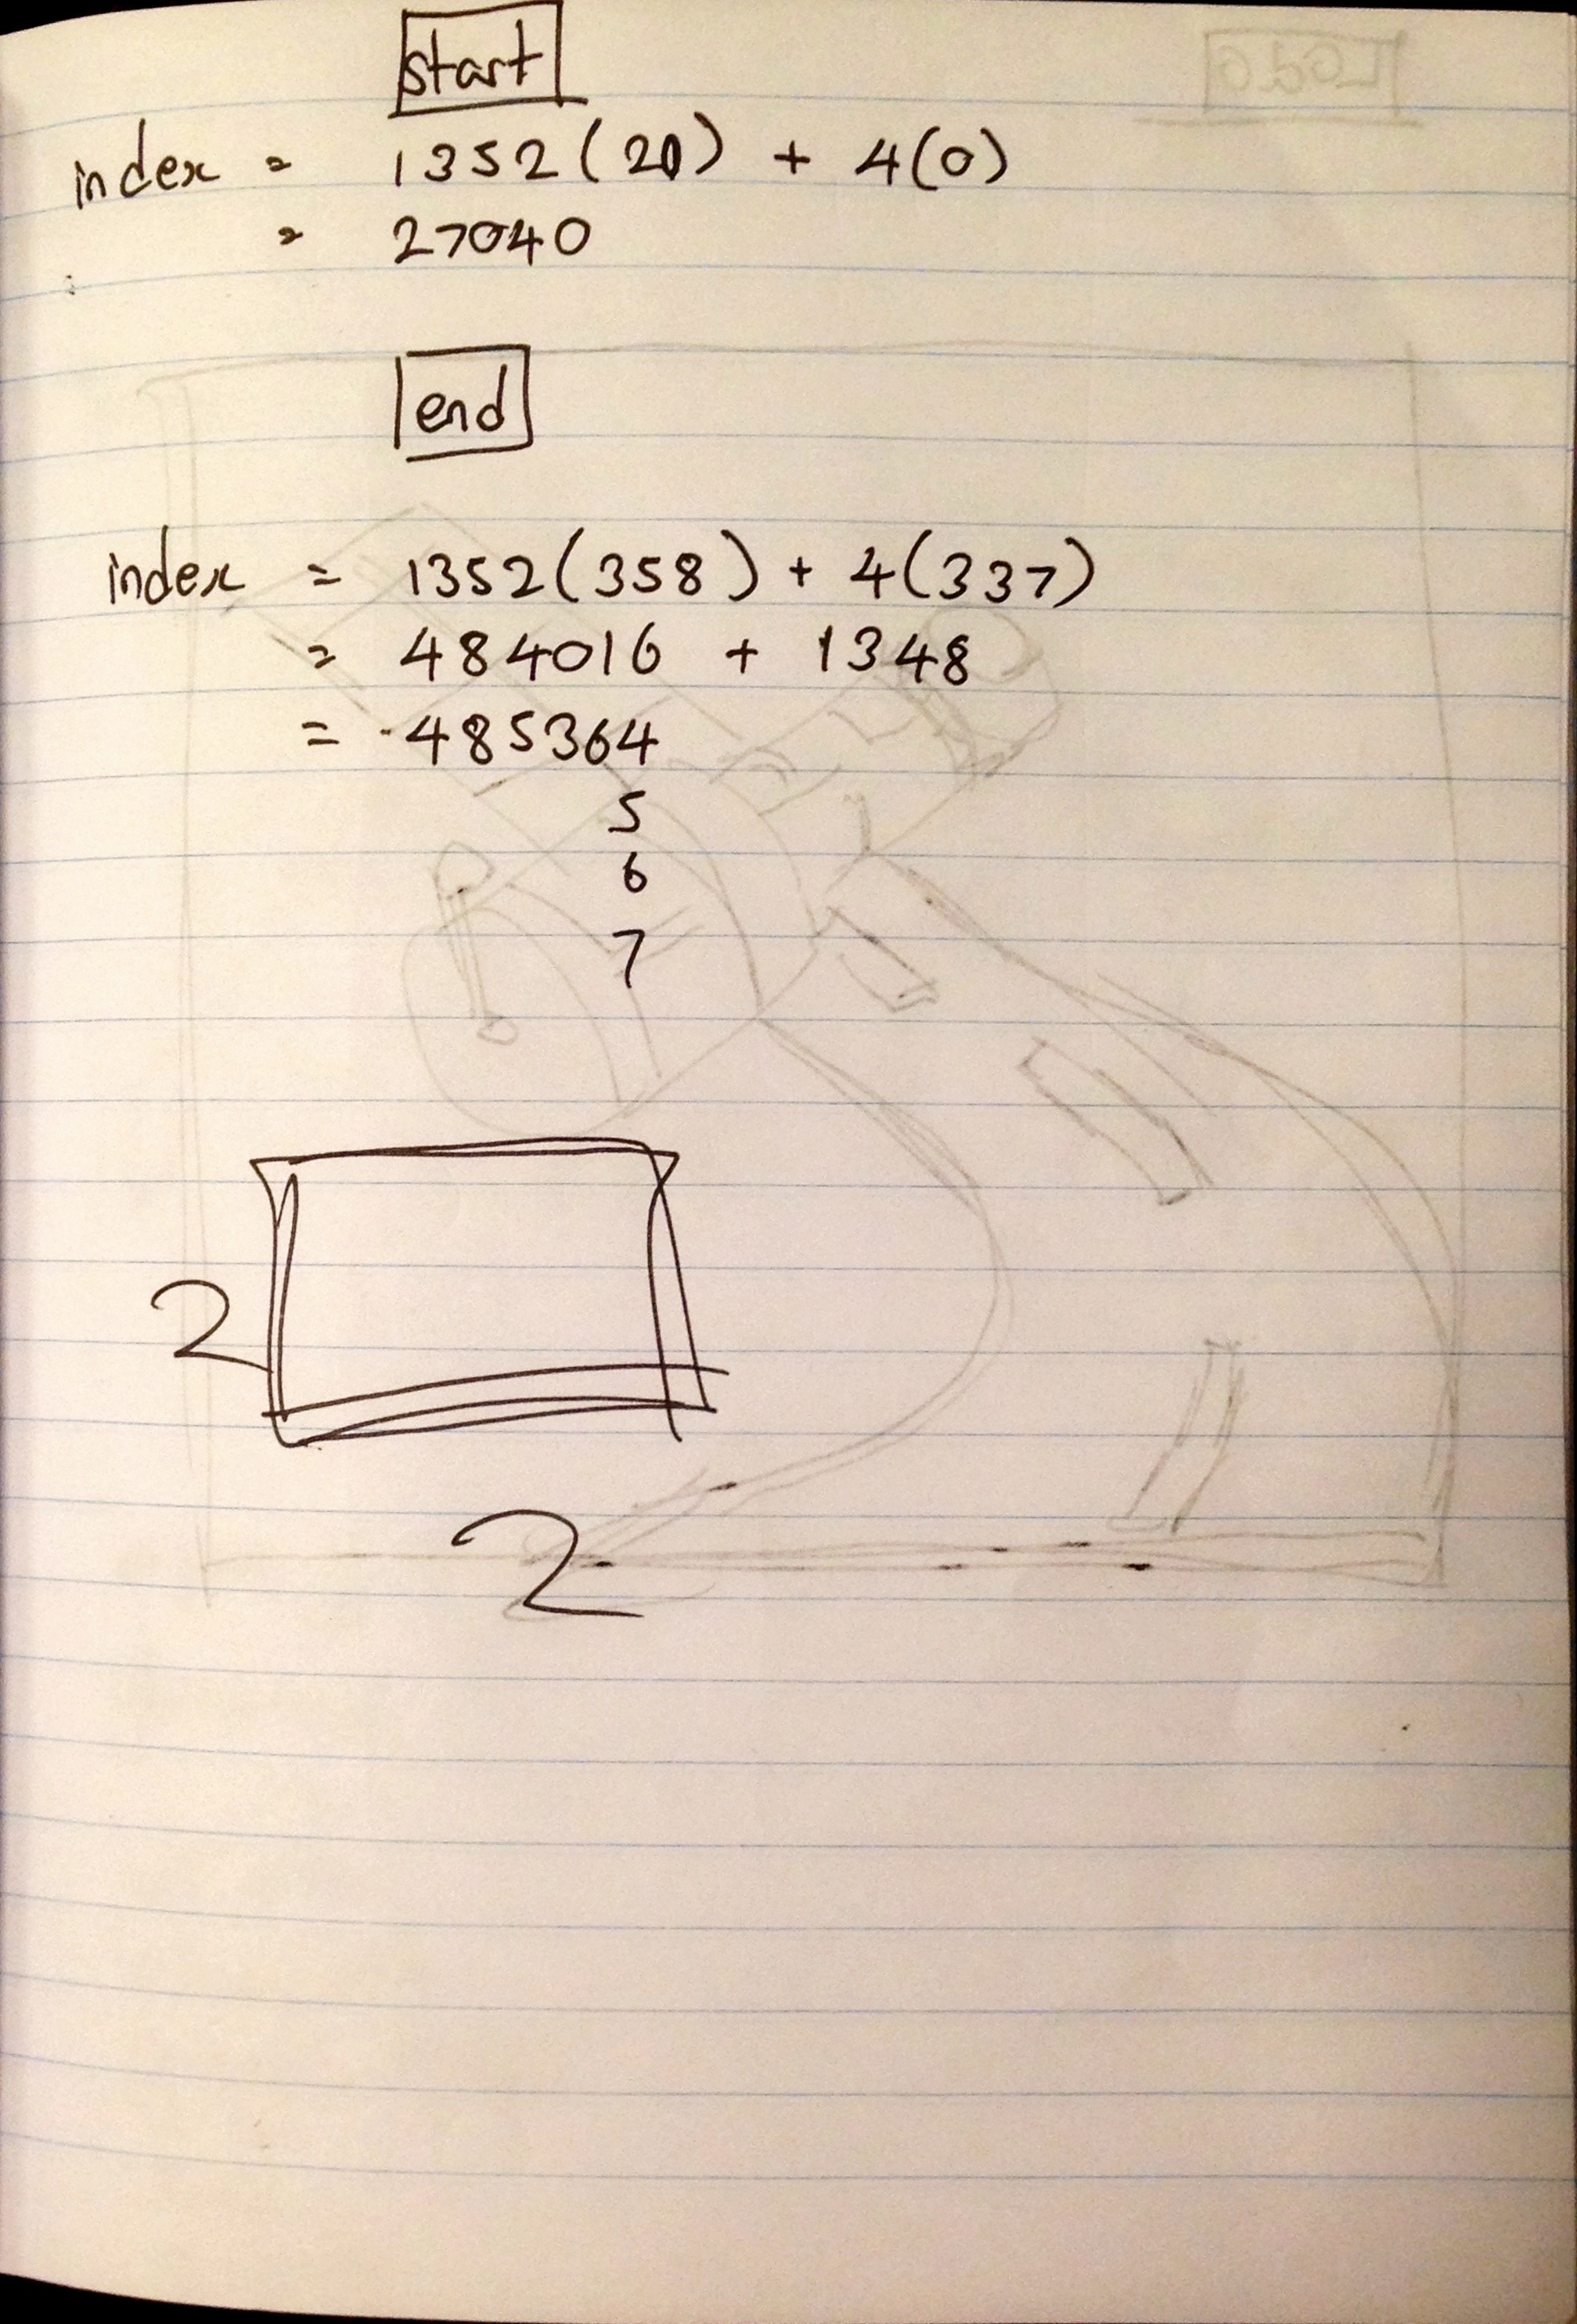
\includegraphics[width=\textwidth]{8.JPG}
		\caption{Image size work process 8.}
	\end{minipage}
\end{figure}

%%%%%%%%%%%%%%%%%%%%%%%%%%%%%%%%%%%%%%%%%%%%%%%%%%%%%%%%%%%%%%%%%%%%%%%%

\chapter{References}
\bibliography{reference/reference}
\bibliographystyle{apalike}

%%%%%%%%%%%%%%%%%%%%%%%%%%%%%%%%%%%%%%%%%%%%%%%%%%%%%%%%%%%%%%%%%%%%%%%%

\end{document}